% Options for packages loaded elsewhere
\PassOptionsToPackage{unicode}{hyperref}
\PassOptionsToPackage{hyphens}{url}
%
\documentclass[
  ignorenonframetext,
]{beamer}
\usepackage{pgfpages}
\setbeamertemplate{caption}[numbered]
\setbeamertemplate{caption label separator}{: }
\setbeamercolor{caption name}{fg=normal text.fg}
\beamertemplatenavigationsymbolsempty
% Prevent slide breaks in the middle of a paragraph
\widowpenalties 1 10000
\raggedbottom
\setbeamertemplate{part page}{
  \centering
  \begin{beamercolorbox}[sep=16pt,center]{part title}
    \usebeamerfont{part title}\insertpart\par
  \end{beamercolorbox}
}
\setbeamertemplate{section page}{
  \centering
  \begin{beamercolorbox}[sep=12pt,center]{part title}
    \usebeamerfont{section title}\insertsection\par
  \end{beamercolorbox}
}
\setbeamertemplate{subsection page}{
  \centering
  \begin{beamercolorbox}[sep=8pt,center]{part title}
    \usebeamerfont{subsection title}\insertsubsection\par
  \end{beamercolorbox}
}
\AtBeginPart{
  \frame{\partpage}
}
\AtBeginSection{
  \ifbibliography
  \else
    \frame{\sectionpage}
  \fi
}
\AtBeginSubsection{
  \frame{\subsectionpage}
}
\usepackage{lmodern}
\usepackage{amssymb,amsmath}
\usepackage{ifxetex,ifluatex}
\ifnum 0\ifxetex 1\fi\ifluatex 1\fi=0 % if pdftex
  \usepackage[T1]{fontenc}
  \usepackage[utf8]{inputenc}
  \usepackage{textcomp} % provide euro and other symbols
\else % if luatex or xetex
  \usepackage{unicode-math}
  \defaultfontfeatures{Scale=MatchLowercase}
  \defaultfontfeatures[\rmfamily]{Ligatures=TeX,Scale=1}
\fi
% Use upquote if available, for straight quotes in verbatim environments
\IfFileExists{upquote.sty}{\usepackage{upquote}}{}
\IfFileExists{microtype.sty}{% use microtype if available
  \usepackage[]{microtype}
  \UseMicrotypeSet[protrusion]{basicmath} % disable protrusion for tt fonts
}{}
\makeatletter
\@ifundefined{KOMAClassName}{% if non-KOMA class
  \IfFileExists{parskip.sty}{%
    \usepackage{parskip}
  }{% else
    \setlength{\parindent}{0pt}
    \setlength{\parskip}{6pt plus 2pt minus 1pt}}
}{% if KOMA class
  \KOMAoptions{parskip=half}}
\makeatother
\usepackage{xcolor}
\IfFileExists{xurl.sty}{\usepackage{xurl}}{} % add URL line breaks if available
\IfFileExists{bookmark.sty}{\usepackage{bookmark}}{\usepackage{hyperref}}
\hypersetup{
  pdftitle={Tema 9 - Datos cuantitativos agrupados},
  pdfauthor={Juan Gabriel Gomila \& María Santos},
  hidelinks,
  pdfcreator={LaTeX via pandoc}}
\urlstyle{same} % disable monospaced font for URLs
\newif\ifbibliography
\usepackage{color}
\usepackage{fancyvrb}
\newcommand{\VerbBar}{|}
\newcommand{\VERB}{\Verb[commandchars=\\\{\}]}
\DefineVerbatimEnvironment{Highlighting}{Verbatim}{commandchars=\\\{\}}
% Add ',fontsize=\small' for more characters per line
\usepackage{framed}
\definecolor{shadecolor}{RGB}{248,248,248}
\newenvironment{Shaded}{\begin{snugshade}}{\end{snugshade}}
\newcommand{\AlertTok}[1]{\textcolor[rgb]{0.94,0.16,0.16}{#1}}
\newcommand{\AnnotationTok}[1]{\textcolor[rgb]{0.56,0.35,0.01}{\textbf{\textit{#1}}}}
\newcommand{\AttributeTok}[1]{\textcolor[rgb]{0.77,0.63,0.00}{#1}}
\newcommand{\BaseNTok}[1]{\textcolor[rgb]{0.00,0.00,0.81}{#1}}
\newcommand{\BuiltInTok}[1]{#1}
\newcommand{\CharTok}[1]{\textcolor[rgb]{0.31,0.60,0.02}{#1}}
\newcommand{\CommentTok}[1]{\textcolor[rgb]{0.56,0.35,0.01}{\textit{#1}}}
\newcommand{\CommentVarTok}[1]{\textcolor[rgb]{0.56,0.35,0.01}{\textbf{\textit{#1}}}}
\newcommand{\ConstantTok}[1]{\textcolor[rgb]{0.00,0.00,0.00}{#1}}
\newcommand{\ControlFlowTok}[1]{\textcolor[rgb]{0.13,0.29,0.53}{\textbf{#1}}}
\newcommand{\DataTypeTok}[1]{\textcolor[rgb]{0.13,0.29,0.53}{#1}}
\newcommand{\DecValTok}[1]{\textcolor[rgb]{0.00,0.00,0.81}{#1}}
\newcommand{\DocumentationTok}[1]{\textcolor[rgb]{0.56,0.35,0.01}{\textbf{\textit{#1}}}}
\newcommand{\ErrorTok}[1]{\textcolor[rgb]{0.64,0.00,0.00}{\textbf{#1}}}
\newcommand{\ExtensionTok}[1]{#1}
\newcommand{\FloatTok}[1]{\textcolor[rgb]{0.00,0.00,0.81}{#1}}
\newcommand{\FunctionTok}[1]{\textcolor[rgb]{0.00,0.00,0.00}{#1}}
\newcommand{\ImportTok}[1]{#1}
\newcommand{\InformationTok}[1]{\textcolor[rgb]{0.56,0.35,0.01}{\textbf{\textit{#1}}}}
\newcommand{\KeywordTok}[1]{\textcolor[rgb]{0.13,0.29,0.53}{\textbf{#1}}}
\newcommand{\NormalTok}[1]{#1}
\newcommand{\OperatorTok}[1]{\textcolor[rgb]{0.81,0.36,0.00}{\textbf{#1}}}
\newcommand{\OtherTok}[1]{\textcolor[rgb]{0.56,0.35,0.01}{#1}}
\newcommand{\PreprocessorTok}[1]{\textcolor[rgb]{0.56,0.35,0.01}{\textit{#1}}}
\newcommand{\RegionMarkerTok}[1]{#1}
\newcommand{\SpecialCharTok}[1]{\textcolor[rgb]{0.00,0.00,0.00}{#1}}
\newcommand{\SpecialStringTok}[1]{\textcolor[rgb]{0.31,0.60,0.02}{#1}}
\newcommand{\StringTok}[1]{\textcolor[rgb]{0.31,0.60,0.02}{#1}}
\newcommand{\VariableTok}[1]{\textcolor[rgb]{0.00,0.00,0.00}{#1}}
\newcommand{\VerbatimStringTok}[1]{\textcolor[rgb]{0.31,0.60,0.02}{#1}}
\newcommand{\WarningTok}[1]{\textcolor[rgb]{0.56,0.35,0.01}{\textbf{\textit{#1}}}}
\usepackage{longtable,booktabs}
\usepackage{caption}
% Make caption package work with longtable
\makeatletter
\def\fnum@table{\tablename~\thetable}
\makeatother
\usepackage{graphicx,grffile}
\makeatletter
\def\maxwidth{\ifdim\Gin@nat@width>\linewidth\linewidth\else\Gin@nat@width\fi}
\def\maxheight{\ifdim\Gin@nat@height>\textheight\textheight\else\Gin@nat@height\fi}
\makeatother
% Scale images if necessary, so that they will not overflow the page
% margins by default, and it is still possible to overwrite the defaults
% using explicit options in \includegraphics[width, height, ...]{}
\setkeys{Gin}{width=\maxwidth,height=\maxheight,keepaspectratio}
% Set default figure placement to htbp
\makeatletter
\def\fps@figure{htbp}
\makeatother
\setlength{\emergencystretch}{3em} % prevent overfull lines
\providecommand{\tightlist}{%
  \setlength{\itemsep}{0pt}\setlength{\parskip}{0pt}}
\setcounter{secnumdepth}{-\maxdimen} % remove section numbering

\title{Tema 9 - Datos cuantitativos agrupados}
\author{Juan Gabriel Gomila \& María Santos}
\date{}

\begin{document}
\frame{\titlepage}

\begin{frame}{Introducción}
\protect\hypertarget{introducciuxf3n}{}

Aunque no seamos completamente conscientes de ello, tendemos a agrupar
datos cuantitativos constantemente.

Sin ir más lejos, calificamos de excelente a todas las notas que están
sobre el 9. También decimos que una persona tiene 20 años cuando se
encuentra en el intervalo {[}20,21). Es decir, cuando ha cumplido los 20
pero aún no tiene los 21.

En estadística, existen innumerables motivos por los cuales nos interesa
agrupar los datos cuando estos son cuantitativos. Uno de estos motivos
puede ser perfectamente que los datos sean muy heterogéneos. En este
caso, nos encontraríamos con que las frecuencias de los valores
individuales serían todas muy similares, lo que daría lugar a un
diagrama de barras muy difícil de interpretar, tal y como mostramos en
el siguiente ejemplo.

\end{frame}

\begin{frame}[fragile]{Ejemplo 1}
\protect\hypertarget{ejemplo-1}{}

\textbf{Ejemplo 1}

Consideremos la siguiente muestra de 24 pesos de estudiantes:

\begin{Shaded}
\begin{Highlighting}[]
\NormalTok{pesos =}\StringTok{ }\KeywordTok{c}\NormalTok{(}\FloatTok{55.2}\NormalTok{,}\FloatTok{54.0}\NormalTok{,}\FloatTok{55.2}\NormalTok{,}\FloatTok{53.7}\NormalTok{,}\FloatTok{60.2}\NormalTok{,}\FloatTok{53.2}\NormalTok{,}\FloatTok{54.6}\NormalTok{,}\FloatTok{55.1}\NormalTok{,}\FloatTok{51.2}\NormalTok{,}\FloatTok{53.2}\NormalTok{,}\FloatTok{54.8}\NormalTok{,}\FloatTok{52.3}\NormalTok{,}\FloatTok{56.9}\NormalTok{,}\FloatTok{57.0}\NormalTok{,}\FloatTok{55.0}\NormalTok{,}
          \FloatTok{53.5}\NormalTok{,}\FloatTok{50.9}\NormalTok{,}\FloatTok{55.1}\NormalTok{,}\FloatTok{53.6}\NormalTok{,}\FloatTok{61.2}\NormalTok{,}\FloatTok{59.5}\NormalTok{,}\FloatTok{50.3}\NormalTok{,}\FloatTok{52.7}\NormalTok{,}\FloatTok{60.0}\NormalTok{)}
\end{Highlighting}
\end{Shaded}

El diagrama de barras de sus frecuencias absolutas, tomando como
posibles niveles todos los pesos entre su mínimo y máximo se muestra en
la siguiente diapositiva.

Como vemos, todas estas frecuencias se encuentran entre 0 y 2, cosa que
no nos da mucha información.

\end{frame}

\begin{frame}[fragile]{Ejemplo 1}
\protect\hypertarget{ejemplo-1-1}{}

\begin{Shaded}
\begin{Highlighting}[]
\KeywordTok{barplot}\NormalTok{(}\KeywordTok{table}\NormalTok{(pesos))}
\end{Highlighting}
\end{Shaded}

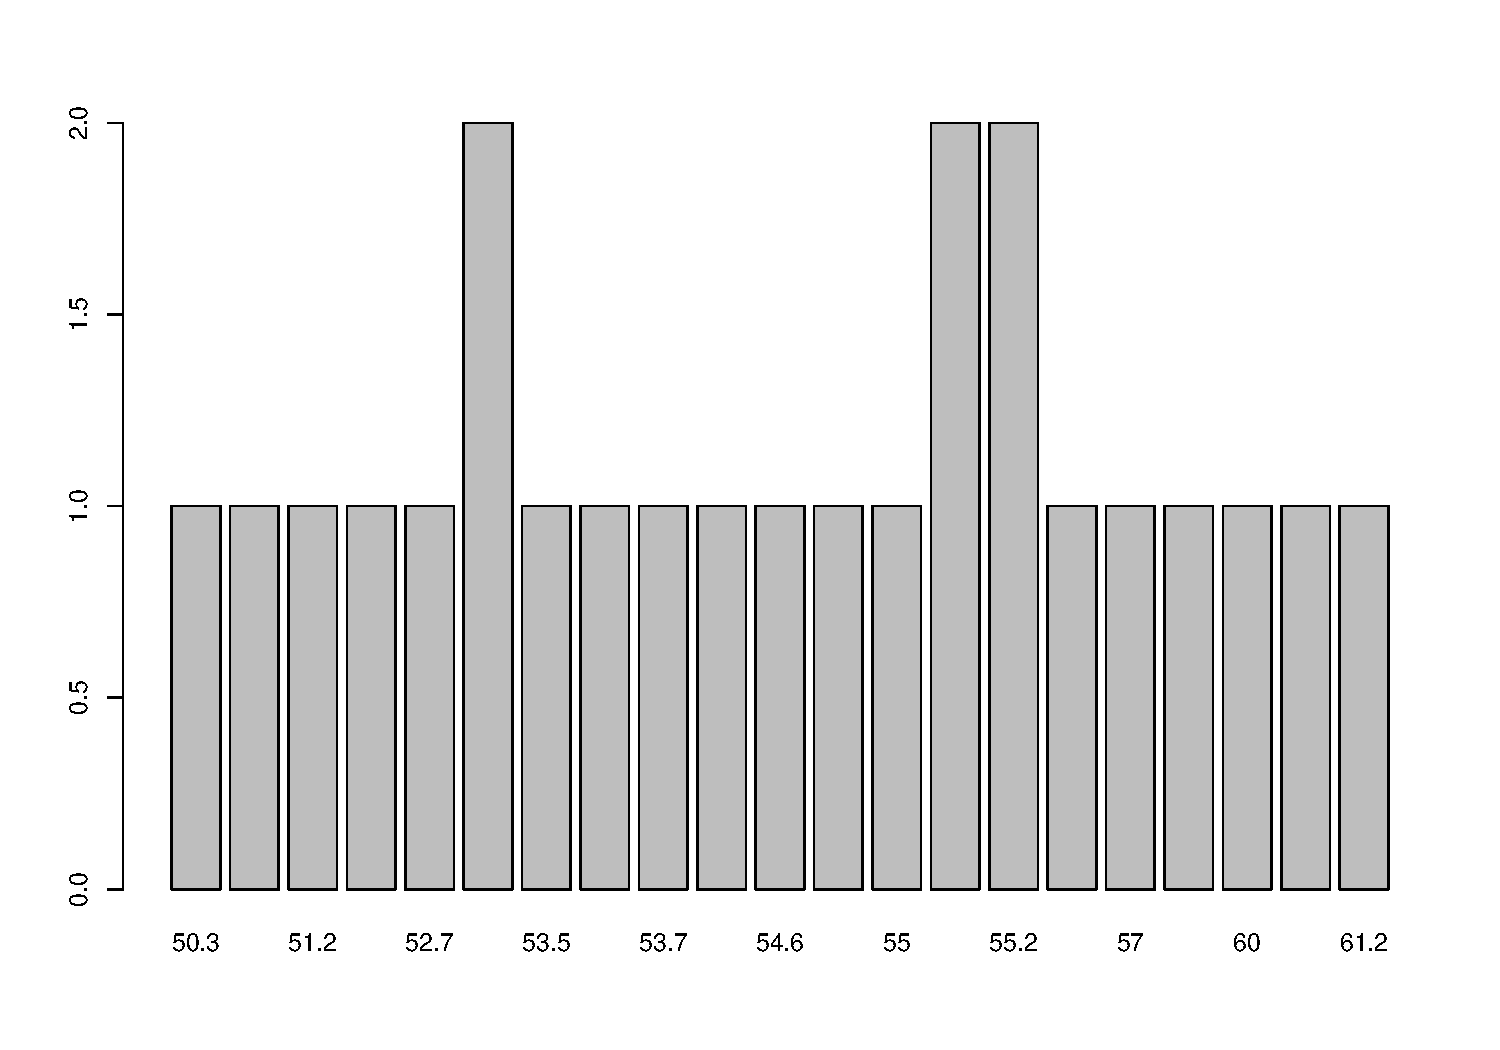
\includegraphics{Tema9.-Agrupacion_datos_cuantitativos_files/figure-beamer/unnamed-chunk-2-1.pdf}

\end{frame}

\begin{frame}{Ejemplo 1}
\protect\hypertarget{ejemplo-1-2}{}

En cambio, si dividiésemos todos estos posibles valores que puede tomar
la variable cuantitativa en intervalos y tomásemos como sus frecuencias
las de todos los valores que caen en dicho intervalo, la cosa cambia.

En este caso, sería mucho más fácil interpretar los resultados, ya que
estos darán mucha más información. Más adelante veremos como crear estos
intervalos.

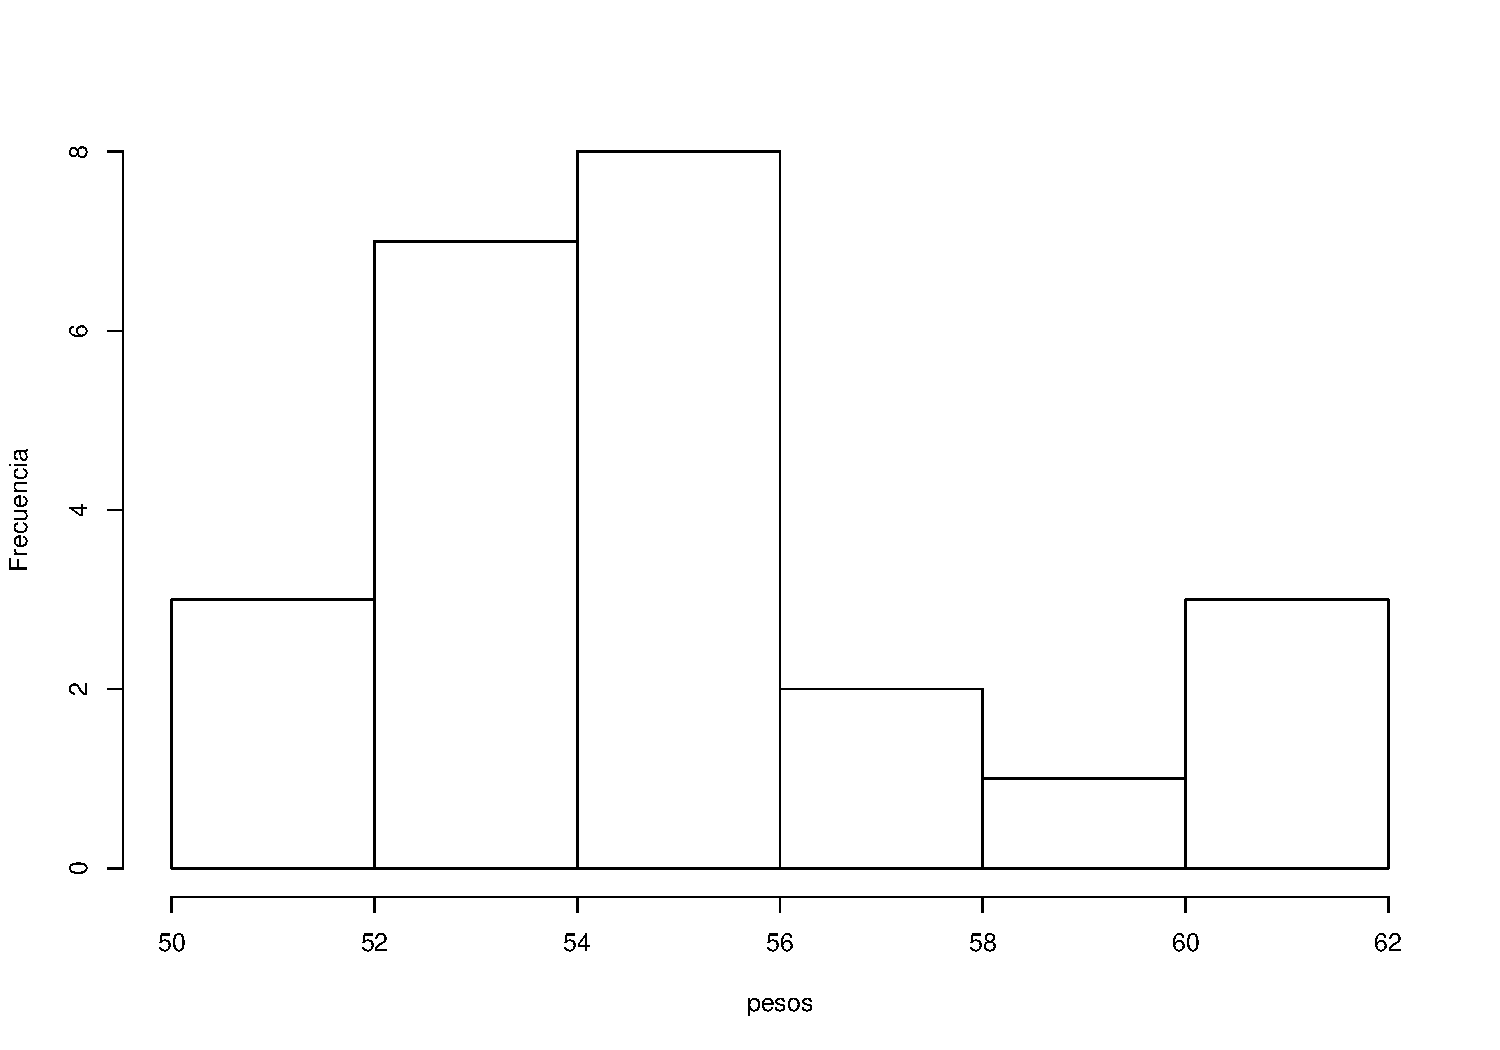
\includegraphics{Tema9.-Agrupacion_datos_cuantitativos_files/figure-beamer/unnamed-chunk-3-1.pdf}

\end{frame}

\begin{frame}{Introducción}
\protect\hypertarget{introducciuxf3n-1}{}

Otro de los motivos por el que necesitamos muchas veces agrupar los
datos cuantitativos es porque, como ya dijimos en temas anteriores, la
precisión infinita no existe. Por tanto, esta imposibilidad de medir de
manera exacta muchas de las magnitudes continuas (tiempo, peso,
altura\ldots) nos obliga a trabajar con aproximaciones o redondeos de
valores reales y que cada uno de estos represente todo un intervalo de
posibles valores.

\end{frame}

\begin{frame}{Introducción}
\protect\hypertarget{introducciuxf3n-2}{}

Por lo general, existen 3 situaciones en las cuales conviene sin lugar a
dudas agrupar datos cuantitativos en intervalos, también llamados clases

\begin{itemize}
\tightlist
\item
  Cuando los datos son continuos, su redondeo ya define un agrupamiento
  debido a la inexistencia de precisión infinita
\item
  Cuando los datos son discretos, pero con un número considerablemente
  grande de posibles valores
\item
  Cuando tenemos muchísimos datos y estamos interesados en estudiar las
  frecuencias de sus valores
\end{itemize}

\end{frame}

\hypertarget{cuxf3mo-agrupar-datos}{%
\section{Cómo agrupar datos}\label{cuxf3mo-agrupar-datos}}

\begin{frame}{Los 4 pasos}
\protect\hypertarget{los-4-pasos}{}

Antes de estudiar unos datos agrupados, hay que, obviamente, agruparlos.
Este proceso consta de 4 pasos:

\begin{enumerate}
\tightlist
\item
  Decidir el número de intervalos que vamos a utilizar
\item
  Decidir la amplitud de estos intervalos
\item
  Acumular los extremos de los intervalos
\item
  Calcular el valor representativo de cada intervalo, su marca de clase
\end{enumerate}

No hay una forma de agrupar datos mejor que otra. Eso sí, cada uno de
los diferentes agrupamientos para un conjunto de datos podría sacar a la
luz características diferentes del conjunto.

\end{frame}

\begin{frame}[fragile]{La función hist()}
\protect\hypertarget{la-funciuxf3n-hist}{}

La función de R por excelencia para estudiar datos agrupados es
\texttt{hist}. Dicha función implementa los 4 pasos del proceso.

Si le indicamos como argumentos el vector de datos y el número de
intervalos que deseamos, o bien el método para determinarlo (cosa que
veremos a continuación), la función agrupará los datos en el número de
clases que le hemos introducido, más o menos. Eso sí, sin control de
ningún tipo por nuestra parte sobre los intervalos que produce.

Esto puede venirnos bien en algunos casos, pero no en otros.

\end{frame}

\begin{frame}{Estableciendo el número de clases}
\protect\hypertarget{estableciendo-el-nuxfamero-de-clases}{}

En este tema explicaremos una receta para agrupar datos. Lo dicho, ni
mejor ni peor que el resto.

Lo primero es establecer el número \(k\) de clases en las que vamos a
dividir nuestros datos. Podemos decidir en función de nuestros intereses
o podemos hacer uso de alguna de las reglas existentes. Destacaremos las
más populares. Sea \(n\) el número total de datos de la muestra

\begin{itemize}
\tightlist
\item
  Regla de la raíz cuadrada: \(k = \lceil\sqrt{n}\ \rceil\)
\item
  Regla de Sturges: \(k = \lceil 1+\log_{2}(n)\rceil\)
\end{itemize}

\end{frame}

\begin{frame}{Estableciendo el número de clases}
\protect\hypertarget{estableciendo-el-nuxfamero-de-clases-1}{}

\begin{itemize}
\tightlist
\item
  Regla de Scott: Se determina primero la amplitud teórica, \(A_S\) de
  las clases \[A_S = 3.5\cdot\tilde{s}\cdot n^{-\frac{1}{3}}\] donde
  \(\tilde{s}\) es la desviación típica muestral. Luego se toma
  \[k = \left\lceil \frac{\max(x)-\min(x)}{A_S}\right\rceil\]
\end{itemize}

\end{frame}

\begin{frame}{Estableciendo el número de clases}
\protect\hypertarget{estableciendo-el-nuxfamero-de-clases-2}{}

\begin{itemize}
\tightlist
\item
  Regla de Freedman-Diaconis: Se determina primero la amplitud teórica,
  \(A_{FD}\) de las clases
  \[A_{FD} = 2\cdot(Q_{0.75}-Q_{0.25})\cdot n^{-\frac{1}{3}}\] (donde,
  recordemos, \(Q_{0.75}-Q_{0.25}\), es el rango intercuantílico) y
  entonces
  \[k = \left\lceil \frac{\max(x)-\min(x)}{A_{FD}}\right\rceil\]
\end{itemize}

Si os fijáis, las dos primeras solo dependen de \(n\), mientras que las
dos últimas también tienen en cuenta, de formas diferentes, la
dispersión de los datos. De nuevo, no hay ninguna mejor que las demás.
Pero sí puede ocurrir que métodos diferentes den lugar a la observación
de características diferentes en los datos.

\end{frame}

\begin{frame}[fragile]{Estableciendo el número de clases con R}
\protect\hypertarget{estableciendo-el-nuxfamero-de-clases-con-r}{}

Las instrucciones para llevar a cabo las 3 últimas reglas con R son,
respectivamente,

\begin{itemize}
\tightlist
\item
  \texttt{nclass.Sturges}
\item
  \texttt{nclass.scott}
\item
  \texttt{nclass.FD}
\end{itemize}

Puede ocurrir que las difrentes reglas den valores diferentes, o no.

\end{frame}

\begin{frame}{Decidiendo la amplitud}
\protect\hypertarget{decidiendo-la-amplitud}{}

Una vez determinado \(k\), hay que decidir su amplitud.

La forma más fácil y la que nosotros utilizaremos por defecto es que la
amplitud de todos los intervalos sea la misma, \(A\). Esta forma no es
la única.

Para calcular \(A\), lo que haremos será dividir el rango de los datos
entre \(k\), el número de clases, y redondearemos por exceso a un valor
de la precisión de la medida.

Si se da el improbable caso en que el cociente de exacto, tomaremos como
\(A\) ese cociente más una unidad de precisión.

\end{frame}

\begin{frame}{Extremos de los intervalos}
\protect\hypertarget{extremos-de-los-intervalos}{}

Es la hora de calcular los extremos de los intervalos. Nosotros
tomaremos estos intervalos siempre cerrados por su izquierda y abiertos
por la derecha, debido a que esta es la forma en que R los construye y
porque es así como se utilizan en Teoría de Probabilidades al definir la
distribución de una variable aleatoria discreta y también en otras
muchas situaciones cotidianas.

Utilizaremos la siguiente notación
\[[L_1,L_2),[L_2,L_3),\dots,[L_k,L_{k+1})\]

donde los \(L_i\) denotan los extremos de los intervalos. Estos se
calculan de la siguiente forma:

\[L_1 = \min(x)-\frac{1}{2}\cdot \text{precisión}\]

\end{frame}

\begin{frame}{Extremos de los intervalos}
\protect\hypertarget{extremos-de-los-intervalos-1}{}

A partir de \(L_1\), el resto de intervalos se obtiene de forma
recursiva: \[L_2 = L_1 + A\] \[L_3 = L_2 + A\] \[\vdots\]
\[L_{k+1} = L_k+A\]

Si nos fijamos bien, los extremos forman una progresión aritmética de
salto \(A\): \[L_{i} = L_{1}+(i-1)A,\qquad i=2,\dots,k+1\]

De esta forma garantizamos que los extremos de los intervalos nunca
coincidan con valores del conjunto de datos, puesto que tinen una
precisión mayor.

\end{frame}

\begin{frame}{Marca de clase}
\protect\hypertarget{marca-de-clase}{}

Solo nos queda determinar la marca de clase, \(X_i\), de cada intervalo
\([L_i,L_{i+1})\).

Este no es más que un valor del intervalo que utilizaremos para
identificar la clase y para calcular algunos estadísticos.

Genralmente, \[X_i = \frac{L_i+L_{i+1}}{2}\] es decir, \(X_i\) será el
punto medio del intervalo, para así garantizar que el error máximo
cometido al describir cualquier elemento del intervalo por medio de su
marca de clase sea mínimo o igual a la mitad de la amplitud del
respectivo intervalo.

\end{frame}

\begin{frame}{Marca de clase}
\protect\hypertarget{marca-de-clase-1}{}

Es sencillo concluir que, al tener todos los intervalos amplitud \(A\),
la distancia entre \(X_i\) y \(X_{i+1}\) tambien será \(A\). Por
consiguiente,

\[X_{i} = X_1+ (i-1)A,\qquad i=2,\dots,k\]

donde \[X_1 = \frac{L_1+L_2}{2}\]

\end{frame}

\hypertarget{ejemplo-2}{%
\section{Ejemplo 2}\label{ejemplo-2}}

\begin{frame}[fragile]{Enunciado}
\protect\hypertarget{enunciado}{}

\textbf{Ejemplo 2}

Vamos a considerar el conjunto de datos de \texttt{datacrab}. Para
nuestro estudio, trabajaremos únicamente con la variable \texttt{width}.

Llevaremos a cabo los 4 pasos explicados con anterioridad: cálculo del
número de intervalos, determinación de la amplitud, cálculo de los
extremos y las marcas de clase.

\end{frame}

\begin{frame}[fragile]{Solución}
\protect\hypertarget{soluciuxf3n}{}

En primer lugar, cargamos los datos en un data frame:

\begin{Shaded}
\begin{Highlighting}[]
\NormalTok{crabs =}\StringTok{ }\KeywordTok{read.table}\NormalTok{(}\StringTok{"../data/datacrab.txt"}\NormalTok{, }\DataTypeTok{header =} \OtherTok{TRUE}\NormalTok{)}
\KeywordTok{str}\NormalTok{(crabs)}
\end{Highlighting}
\end{Shaded}

\begin{verbatim}
'data.frame':   173 obs. of  6 variables:
 $ input : int  1 2 3 4 5 6 7 8 9 10 ...
 $ color : int  3 4 2 4 4 3 2 4 3 4 ...
 $ spine : int  3 3 1 3 3 3 1 2 1 3 ...
 $ width : num  28.3 22.5 26 24.8 26 23.8 26.5 24.7 23.7 25.6 ...
 $ satell: int  8 0 9 0 4 0 0 0 0 0 ...
 $ weight: int  3050 1550 2300 2100 2600 2100 2350 1900 1950 2150 ...
\end{verbatim}

\begin{Shaded}
\begin{Highlighting}[]
\NormalTok{cw =}\StringTok{ }\NormalTok{crabs}\OperatorTok{$}\NormalTok{width}
\end{Highlighting}
\end{Shaded}

A continuación, definimos la variable \texttt{cw} que contiene los datos
de la variable \texttt{width}.

\end{frame}

\begin{frame}[fragile]{Solución}
\protect\hypertarget{soluciuxf3n-1}{}

Calculemos el número de clases según las diferentes reglas que hemos
visto:

\begin{itemize}
\tightlist
\item
  Regla de la raíz cuadrada:
\end{itemize}

\begin{Shaded}
\begin{Highlighting}[]
\NormalTok{n =}\StringTok{ }\KeywordTok{length}\NormalTok{(cw)}
\NormalTok{k1 =}\StringTok{ }\KeywordTok{ceiling}\NormalTok{(}\KeywordTok{sqrt}\NormalTok{(n))}
\NormalTok{k1}
\end{Highlighting}
\end{Shaded}

\begin{verbatim}
[1] 14
\end{verbatim}

\begin{itemize}
\tightlist
\item
  Regla de Sturges:
\end{itemize}

\begin{Shaded}
\begin{Highlighting}[]
\NormalTok{k2 =}\StringTok{ }\KeywordTok{ceiling}\NormalTok{(}\DecValTok{1}\OperatorTok{+}\KeywordTok{log}\NormalTok{(n,}\DecValTok{2}\NormalTok{))}
\NormalTok{k2}
\end{Highlighting}
\end{Shaded}

\begin{verbatim}
[1] 9
\end{verbatim}

\end{frame}

\begin{frame}[fragile]{Solución}
\protect\hypertarget{soluciuxf3n-2}{}

\begin{itemize}
\tightlist
\item
  Regla de Scott:
\end{itemize}

\begin{Shaded}
\begin{Highlighting}[]
\NormalTok{As =}\StringTok{ }\FloatTok{3.5}\OperatorTok{*}\KeywordTok{sd}\NormalTok{(cw)}\OperatorTok{*}\NormalTok{n}\OperatorTok{^}\NormalTok{(}\OperatorTok{-}\DecValTok{1}\OperatorTok{/}\DecValTok{3}\NormalTok{) }\CommentTok{#Amplitud teórica}
\NormalTok{k3 =}\StringTok{ }\KeywordTok{ceiling}\NormalTok{(}\KeywordTok{diff}\NormalTok{(}\KeywordTok{range}\NormalTok{(cw))}\OperatorTok{/}\NormalTok{As)}
\NormalTok{k3}
\end{Highlighting}
\end{Shaded}

\begin{verbatim}
[1] 10
\end{verbatim}

\begin{itemize}
\tightlist
\item
  Regla de Freedman-Diaconis:
\end{itemize}

\begin{Shaded}
\begin{Highlighting}[]
\CommentTok{#Amplitud teórica}
\NormalTok{Afd =}\StringTok{ }\DecValTok{2}\OperatorTok{*}\NormalTok{(}\KeywordTok{quantile}\NormalTok{(cw,}\FloatTok{0.75}\NormalTok{, }\DataTypeTok{names =} \OtherTok{FALSE}\NormalTok{)}\OperatorTok{-}\KeywordTok{quantile}\NormalTok{(cw,}\FloatTok{0.25}\NormalTok{,}\DataTypeTok{names =} \OtherTok{FALSE}\NormalTok{))}\OperatorTok{*}\NormalTok{n}\OperatorTok{^}\NormalTok{(}\OperatorTok{-}\DecValTok{1}\OperatorTok{/}\DecValTok{3}\NormalTok{) }
\NormalTok{k4 =}\StringTok{ }\KeywordTok{ceiling}\NormalTok{(}\KeywordTok{diff}\NormalTok{(}\KeywordTok{range}\NormalTok{(cw))}\OperatorTok{/}\NormalTok{Afd)}
\NormalTok{k4}
\end{Highlighting}
\end{Shaded}

\begin{verbatim}
[1] 13
\end{verbatim}

\end{frame}

\begin{frame}[fragile]{Solución}
\protect\hypertarget{soluciuxf3n-3}{}

Podemos comprobar nuestros 3 últimos resultados con R:

\begin{Shaded}
\begin{Highlighting}[]
\KeywordTok{nclass.Sturges}\NormalTok{(cw)}
\end{Highlighting}
\end{Shaded}

\begin{verbatim}
[1] 9
\end{verbatim}

\begin{Shaded}
\begin{Highlighting}[]
\KeywordTok{nclass.scott}\NormalTok{(cw)}
\end{Highlighting}
\end{Shaded}

\begin{verbatim}
[1] 10
\end{verbatim}

\begin{Shaded}
\begin{Highlighting}[]
\KeywordTok{nclass.FD}\NormalTok{(cw)}
\end{Highlighting}
\end{Shaded}

\begin{verbatim}
[1] 13
\end{verbatim}

De momento, vamos a seguir la Regla de Scott. Es decir, vamos a
considerar 10 intervalos.

\end{frame}

\begin{frame}[fragile]{Solución}
\protect\hypertarget{soluciuxf3n-4}{}

A continuación, debemos elegir la amplitud de los intervalos.

\begin{Shaded}
\begin{Highlighting}[]
\NormalTok{A =}\StringTok{ }\KeywordTok{diff}\NormalTok{(}\KeywordTok{range}\NormalTok{(cw)) }\OperatorTok{/}\StringTok{ }\DecValTok{10}
\NormalTok{A}
\end{Highlighting}
\end{Shaded}

\begin{verbatim}
[1] 1.25
\end{verbatim}

Como nuestros datos están expresados en mm con una precisión de una
cifra decimal, debemos redondear por exceso a un cifra decimal el
resultado obtenido. Por lo tanto, nuestra amplitud será de

\begin{Shaded}
\begin{Highlighting}[]
\NormalTok{A =}\StringTok{ }\FloatTok{1.3}
\end{Highlighting}
\end{Shaded}

Recordad que si el cociente nos hubiera dado un valor exacto con
respecto a la precisión, tendríamos que haberle sumado una unidad de
precisión.

\end{frame}

\begin{frame}[fragile]{Solución}
\protect\hypertarget{soluciuxf3n-5}{}

Ahora nos toca calcular los extremos \(L_1,\dots,L_{11}\) de los
intervalos.

Recordad que nuestros intervalos tendrán la siguiente forma:

\[[L_1,L_2),\ \dots,\ [L_{10},L_{11})\] Calculamos el primer extremo:

\begin{Shaded}
\begin{Highlighting}[]
\NormalTok{L1 =}\StringTok{ }\KeywordTok{min}\NormalTok{(cw)}\OperatorTok{-}\DecValTok{1}\OperatorTok{/}\DecValTok{2}\OperatorTok{*}\FloatTok{0.1}
\NormalTok{L1}
\end{Highlighting}
\end{Shaded}

\begin{verbatim}
[1] 20.95
\end{verbatim}

donde 0.1 es nuestra precisión (décimas de unidad, en este caso).

\end{frame}

\begin{frame}[fragile]{Solución}
\protect\hypertarget{soluciuxf3n-6}{}

Y, el resto de extremos se calculan del siguiente modo:

\begin{Shaded}
\begin{Highlighting}[]
\NormalTok{L2 =}\StringTok{ }\NormalTok{L1 }\OperatorTok{+}\StringTok{ }\NormalTok{A}
\NormalTok{L3 =}\StringTok{ }\NormalTok{L2 }\OperatorTok{+}\StringTok{ }\NormalTok{A}
\NormalTok{L4 =}\StringTok{ }\NormalTok{L3 }\OperatorTok{+}\StringTok{ }\NormalTok{A}
\NormalTok{L5 =}\StringTok{ }\NormalTok{L4 }\OperatorTok{+}\StringTok{ }\NormalTok{A}
\NormalTok{L6 =}\StringTok{ }\NormalTok{L5 }\OperatorTok{+}\StringTok{ }\NormalTok{A}
\NormalTok{L7 =}\StringTok{ }\NormalTok{L6 }\OperatorTok{+}\StringTok{ }\NormalTok{A}
\NormalTok{L8 =}\StringTok{ }\NormalTok{L7 }\OperatorTok{+}\StringTok{ }\NormalTok{A}
\NormalTok{L9 =}\StringTok{ }\NormalTok{L8 }\OperatorTok{+}\StringTok{ }\NormalTok{A}
\NormalTok{L10 =}\StringTok{ }\NormalTok{L9 }\OperatorTok{+}\StringTok{ }\NormalTok{A}
\NormalTok{L11 =}\StringTok{ }\NormalTok{L10 }\OperatorTok{+}\StringTok{ }\NormalTok{A}
\NormalTok{L =}\StringTok{ }\KeywordTok{c}\NormalTok{(L1,L2,L3,L4,L5,L6,L7,L8,L9,L10,L11)}
\NormalTok{L}
\end{Highlighting}
\end{Shaded}

\begin{verbatim}
 [1] 20.95 22.25 23.55 24.85 26.15 27.45 28.75 30.05 31.35 32.65 33.95
\end{verbatim}

\end{frame}

\begin{frame}[fragile]{Solución}
\protect\hypertarget{soluciuxf3n-7}{}

O bien, si queremos facilitarnos el trabajo, también los podemos
calcular mucho más rápido del siguiente modo:

\begin{Shaded}
\begin{Highlighting}[]
\NormalTok{L =}\StringTok{ }\NormalTok{L1 }\OperatorTok{+}\StringTok{ }\NormalTok{A}\OperatorTok{*}\NormalTok{(}\DecValTok{0}\OperatorTok{:}\DecValTok{10}\NormalTok{)}
\NormalTok{L}
\end{Highlighting}
\end{Shaded}

\begin{verbatim}
 [1] 20.95 22.25 23.55 24.85 26.15 27.45 28.75 30.05 31.35 32.65 33.95
\end{verbatim}

Así, nuestros intervalos serán los siguientes:

\[[20.95,22.25),\ [22.25,23.55),\ [23.55,24.85),\ [24.85,26.15),\ [26.15,27.45),\]
\[[27.45,28.75),\ [28.75,30.05),\ [30.05,31.35),\ [31.35,32.65),\ [32.65,33.95)\]

\end{frame}

\begin{frame}[fragile]{Solución}
\protect\hypertarget{soluciuxf3n-8}{}

Y hemos llegado al úlitmo paso: calcular las marcas de clase.

Recordemos que
\(X_i = \frac{L_{i}+L_{i+1}}{2} \quad\forall i=1,\dots,10\)

Empecemos calculando \(X_1\)

\begin{Shaded}
\begin{Highlighting}[]
\NormalTok{X1 =}\StringTok{ }\NormalTok{(L[}\DecValTok{1}\NormalTok{]}\OperatorTok{+}\NormalTok{L[}\DecValTok{2}\NormalTok{])}\OperatorTok{/}\DecValTok{2}
\NormalTok{X1}
\end{Highlighting}
\end{Shaded}

\begin{verbatim}
[1] 21.6
\end{verbatim}

\end{frame}

\begin{frame}[fragile]{Solución}
\protect\hypertarget{soluciuxf3n-9}{}

Y, el resto de marcas de clase se calculan del siguiente modo:

\begin{Shaded}
\begin{Highlighting}[]
\NormalTok{X2 =}\StringTok{ }\NormalTok{X1 }\OperatorTok{+}\StringTok{ }\NormalTok{A}
\NormalTok{X3 =}\StringTok{ }\NormalTok{X2 }\OperatorTok{+}\StringTok{ }\NormalTok{A}
\NormalTok{X4 =}\StringTok{ }\NormalTok{X3 }\OperatorTok{+}\StringTok{ }\NormalTok{A}
\NormalTok{X5 =}\StringTok{ }\NormalTok{X4 }\OperatorTok{+}\StringTok{ }\NormalTok{A}
\NormalTok{X6 =}\StringTok{ }\NormalTok{X5 }\OperatorTok{+}\StringTok{ }\NormalTok{A}
\NormalTok{X7 =}\StringTok{ }\NormalTok{X6 }\OperatorTok{+}\StringTok{ }\NormalTok{A}
\NormalTok{X8 =}\StringTok{ }\NormalTok{X7 }\OperatorTok{+}\StringTok{ }\NormalTok{A}
\NormalTok{X9 =}\StringTok{ }\NormalTok{X8 }\OperatorTok{+}\StringTok{ }\NormalTok{A}
\NormalTok{X10 =}\StringTok{ }\NormalTok{X9 }\OperatorTok{+}\StringTok{ }\NormalTok{A}
\NormalTok{X =}\StringTok{ }\KeywordTok{c}\NormalTok{(X1,X2,X3,X4,X5,X6,X7,X8,X9,X10)}
\NormalTok{X}
\end{Highlighting}
\end{Shaded}

\begin{verbatim}
 [1] 21.6 22.9 24.2 25.5 26.8 28.1 29.4 30.7 32.0 33.3
\end{verbatim}

\end{frame}

\begin{frame}[fragile]{Solución}
\protect\hypertarget{soluciuxf3n-10}{}

O bien, si queremos facilitarnos el trabajo, también los podemos
calcular mucho más rápido como sucesión:

\begin{Shaded}
\begin{Highlighting}[]
\NormalTok{X =}\StringTok{ }\NormalTok{X1 }\OperatorTok{+}\StringTok{ }\NormalTok{A}\OperatorTok{*}\NormalTok{(}\DecValTok{0}\OperatorTok{:}\DecValTok{9}\NormalTok{)}
\NormalTok{X}
\end{Highlighting}
\end{Shaded}

\begin{verbatim}
 [1] 21.6 22.9 24.2 25.5 26.8 28.1 29.4 30.7 32.0 33.3
\end{verbatim}

o también, como punto medio del intervalo

\begin{Shaded}
\begin{Highlighting}[]
\NormalTok{X =}\StringTok{ }\NormalTok{(L[}\DecValTok{1}\OperatorTok{:}\KeywordTok{length}\NormalTok{(L)}\OperatorTok{-}\DecValTok{1}\NormalTok{]}\OperatorTok{+}\NormalTok{L[}\DecValTok{2}\OperatorTok{:}\KeywordTok{length}\NormalTok{(L)])}\OperatorTok{/}\DecValTok{2}
\NormalTok{X}
\end{Highlighting}
\end{Shaded}

\begin{verbatim}
 [1] 21.6 22.9 24.2 25.5 26.8 28.1 29.4 30.7 32.0 33.3
\end{verbatim}

\end{frame}

\begin{frame}{Ejercicio}
\protect\hypertarget{ejercicio}{}

Repetir este proceso para el número de clases obtenido con

\begin{itemize}
\tightlist
\item
  la regla de la raíz
\item
  la regla de Sturges
\item
  la regla de Freedman-Diaconis
\end{itemize}

\end{frame}

\hypertarget{agrupando-datos-con-r}{%
\section{Agrupando datos con R}\label{agrupando-datos-con-r}}

\begin{frame}{Agrupando los datos con R}
\protect\hypertarget{agrupando-los-datos-con-r}{}

Al agrupar los datos, lo que hacemos es convertir nuestra variable
cuantitativa en un factor cuyos niveles son las clases en que ha sido
dividida e identificamos cada dato con su clase.

A la hora de etiquetar los niveles, podemos elegir 3 codificaciones:

\begin{itemize}
\tightlist
\item
  Los intervalos
\item
  Las marcas de clase (el punto medio de cada intervalo)
\item
  El número de orden de cada intervalo
\end{itemize}

\end{frame}

\begin{frame}[fragile]{La función cut}
\protect\hypertarget{la-funciuxf3n-cut}{}

Esta función es la básica en R para agrupar un vector de datos numéricos
y codificar sus valores con clases a las que pertenecen.

Su sintaxis básica es

\texttt{cut(x,\ breaks=...,\ labels=...,\ right=...)}

\begin{itemize}
\tightlist
\item
  \texttt{x} es el vector numérico, nuestra variable cuantitativa
\item
  \texttt{breaks} puede ser un vector numérico formado por los extremos
  de los intervalos en los que queremos agrupar nuestros datos y que
  habremos calculado previamente. También puede ser un número \(k\), en
  cuyo caso R agrupa los datos en \(k\) clases. Para este caso, R divide
  el intervalo comprendido entre los valores mínimo y máximo de \(x\) en
  \(k\) intervalos y, a continuación, desplaza ligeramente el extremo
  inferior del primer intervalo a la izquierda y el extremo del último,
  a la derecha.
\end{itemize}

\end{frame}

\begin{frame}[fragile]{La función cut}
\protect\hypertarget{la-funciuxf3n-cut-1}{}

\begin{itemize}
\tightlist
\item
  \texttt{labels} es un vector con las etiquetas de los intervalos. Su
  valor por defecto es utilizar la etiqueta de los mismos intervalos. Si
  especificamos \texttt{labels\ =\ FALSE}, obtendremos los intervalos
  etiquetados por medio de los números naturales correlativos, empezando
  por 1. Para utilizar como etiqueta las marcas de clase o cualquier
  otra codificación, hay que entrarlo como valor de este parámetro.
\item
  \texttt{right} es un parámetro que igualadao a \texttt{FALSE} hace que
  los intervalos que consideremos sean cerrados por la izquierda y
  abiertos por la derecha. Este no es su valor por defecto.
\item
  \texttt{include.lowest} igualdo a \texttt{TRUE} combinado con
  \texttt{right\ =\ FALSE} hace que el último intervalo sea cerrado.
  Puede sernos útil en algunos casos.
\end{itemize}

\end{frame}

\begin{frame}[fragile]{La función cut}
\protect\hypertarget{la-funciuxf3n-cut-2}{}

En cualquier caso, el resultado de la función \texttt{cut} es una lista
con los elementos del vector original codificados con las etiquetas de
las clases a las que pertenecen. Bien puede ser un factor o un vector.

\end{frame}

\hypertarget{estudiando-datos-agrupados}{%
\section{Estudiando datos agrupados}\label{estudiando-datos-agrupados}}

\begin{frame}{Frecuencias}
\protect\hypertarget{frecuencias}{}

Una primera consideración es tratar las clases obtenidas en el paso
anterior como los niveles de una variable ordinal y calcular sus
frecuencias.

\begin{itemize}
\tightlist
\item
  La frecuencia absoluta de una clase será el número de datos originales
  que pertenecen a la clase
\item
  La frecuencia absoluta acumulada de una clase será el número de datos
  que pertenecen a dicha clase o alguna de las anteriores
\end{itemize}

\end{frame}

\begin{frame}{Tabla de frecuencias}
\protect\hypertarget{tabla-de-frecuencias}{}

Normalmente, las frecuencias de un conjunto de datos agrupados se suele
representar de la siguiente forma

\begin{longtable}[]{@{}llllll@{}}
\toprule
Intervalos & \(X_j\) & \(n_j\) & \(N_j\) & \(f_j\) &
\(F_j\)\tabularnewline
\midrule
\endhead
\([L_1,L_2)\) & \(X_1\) & \(n_1\) & \(N_1\) & \(f_1\) &
\(F_1\)\tabularnewline
\([L_2,L_3)\) & \(X_2\) & \(n_2\) & \(N_2\) & \(f_2\) &
\(F_2\)\tabularnewline
\(\vdots\) & \(\vdots\) & \(\vdots\) & \(\vdots\) & \(\vdots\) &
\(\vdots\)\tabularnewline
\([L_k,L_{k+1})\) & \(X_k\) & \(n_k\) & \(N_k\) & \(f_k\) &
\(F_k\)\tabularnewline
\bottomrule
\end{longtable}

\end{frame}

\begin{frame}[fragile]{La función hist}
\protect\hypertarget{la-funciuxf3n-hist-1}{}

El cálculo de las frecuencias con R podemos hacerlo mediante las
funciones \texttt{table}, \texttt{prop.table} y \texttt{cumsum}.

También podemos utilizar la función \texttt{hist}, que internamente
genera una list cuya componente \texttt{count} es el vector de
frecuencias absolutas de las clases. Por consiguiente, para calcular
estas frecuencias, podemos utilizar la sintaxis

\texttt{hist(x,\ breaks=...,\ right=FALSE,\ plot=FALSE)\$count}

Conviene igualar el parámetro \texttt{breaks} al vector de los extremos
del intervalo debido a que \texttt{cut} y \texttt{hist} hacen uso de
diferentes métodos para agrupar los datos cuando se especifica solamente
el número \(k\) de clases.

El resultado de \texttt{hist} incluye la componente \texttt{mids} que
contiene el vector de puntos medios de los intervalos, es decir,
nuestras marcas de clase.

\end{frame}

\begin{frame}[fragile]{Tabla de frecuencias con R}
\protect\hypertarget{tabla-de-frecuencias-con-r}{}

Podemos automatizar el cálculo de la ya tan mencionada tabla de
frecuencias, utilizando las dos funciones que mostramos a continuación.

La primera sirve en el caso en que vayamos a tomar todas las clases de
la misma amplitud. Sus parámetros son: \(x\), el vector con los datos
cuantitativos; \(k\), el número de clases; \(A\), su amplitud; y \(p\),
la precisión de los datos (p = 1 si la precisión son unidades, p = 0.1
si la precisión son décimas de unidad\ldots).

Por su parte, la segunda es para cuando conocemos los extremos de las
clases. Sus parámetros son: \(x\), el vector con los datos
cuantitativos; \(L\), el vector de extremos de clases; y \(V\) , un
valor lógico, que ha de ser \texttt{TRUE} si queremos que el último
intervalo sea cerrado, y \texttt{FALSE} en caso contrario.

\end{frame}

\begin{frame}[fragile]{Tablas de frecuencias con R}
\protect\hypertarget{tablas-de-frecuencias-con-r}{}

\begin{Shaded}
\begin{Highlighting}[]
\CommentTok{#Primera función}
\NormalTok{TablaFrecs =}\StringTok{ }\ControlFlowTok{function}\NormalTok{(x,k,A,p)\{ }
\NormalTok{  L =}\StringTok{ }\KeywordTok{min}\NormalTok{(x)}\OperatorTok{-}\NormalTok{p}\OperatorTok{/}\DecValTok{2}\OperatorTok{+}\NormalTok{A}\OperatorTok{*}\NormalTok{(}\DecValTok{0}\OperatorTok{:}\NormalTok{k)}
\NormalTok{  x_cut =}\StringTok{ }\KeywordTok{cut}\NormalTok{(x, }\DataTypeTok{breaks =}\NormalTok{ L, }\DataTypeTok{right=}\OtherTok{FALSE}\NormalTok{)}
\NormalTok{  intervals =}\StringTok{ }\KeywordTok{levels}\NormalTok{(x_cut)}
\NormalTok{  mc =}\StringTok{ }\NormalTok{(L[}\DecValTok{1}\NormalTok{]}\OperatorTok{+}\NormalTok{L[}\DecValTok{2}\NormalTok{])}\OperatorTok{/}\DecValTok{2}\OperatorTok{+}\NormalTok{A}\OperatorTok{*}\NormalTok{(}\DecValTok{0}\OperatorTok{:}\NormalTok{(k}\DecValTok{-1}\NormalTok{))}
\NormalTok{  Fr.abs =}\StringTok{ }\KeywordTok{as.vector}\NormalTok{(}\KeywordTok{table}\NormalTok{(x_cut)) }
\NormalTok{  Fr.rel =}\StringTok{ }\KeywordTok{round}\NormalTok{(Fr.abs}\OperatorTok{/}\KeywordTok{length}\NormalTok{(x),}\DecValTok{4}\NormalTok{) }
\NormalTok{  Fr.cum.abs =}\StringTok{ }\KeywordTok{cumsum}\NormalTok{(Fr.abs) }
\NormalTok{  Fr.cum.rel =}\StringTok{ }\KeywordTok{cumsum}\NormalTok{(Fr.rel)}
\NormalTok{  tabla =}\StringTok{ }\KeywordTok{data.frame}\NormalTok{(intervals, mc, Fr.abs, Fr.cum.abs, Fr.rel, Fr.cum.rel)}
\NormalTok{  tabla}
\NormalTok{  \}}
\end{Highlighting}
\end{Shaded}

\end{frame}

\begin{frame}[fragile]{Tablas de frecuencias}
\protect\hypertarget{tablas-de-frecuencias}{}

\begin{Shaded}
\begin{Highlighting}[]
\NormalTok{TablaFrecs.L =}\StringTok{ }\ControlFlowTok{function}\NormalTok{(x,L,V)\{}
\NormalTok{  x_cut =}\StringTok{ }\KeywordTok{cut}\NormalTok{(x, }\DataTypeTok{breaks=}\NormalTok{L, }\DataTypeTok{right=}\OtherTok{FALSE}\NormalTok{, }\DataTypeTok{include.lowest=}\NormalTok{V)}
\NormalTok{  intervals =}\StringTok{ }\KeywordTok{levels}\NormalTok{(x_cut)}
\NormalTok{  mc =}\StringTok{ }\NormalTok{(L[}\DecValTok{1}\OperatorTok{:}\NormalTok{(}\KeywordTok{length}\NormalTok{(L)}\OperatorTok{-}\DecValTok{1}\NormalTok{)]}\OperatorTok{+}\NormalTok{L[}\DecValTok{2}\OperatorTok{:}\KeywordTok{length}\NormalTok{(L)])}\OperatorTok{/}\DecValTok{2}
\NormalTok{  Fr.abs =}\StringTok{ }\KeywordTok{as.vector}\NormalTok{(}\KeywordTok{table}\NormalTok{(x_cut)) }
\NormalTok{  Fr.rel =}\StringTok{ }\KeywordTok{round}\NormalTok{(Fr.abs}\OperatorTok{/}\KeywordTok{length}\NormalTok{(x),}\DecValTok{4}\NormalTok{)}
\NormalTok{  Fr.cum.abs =}\StringTok{ }\KeywordTok{cumsum}\NormalTok{(Fr.abs)}
\NormalTok{  Fr.cum.rel =}\StringTok{ }\KeywordTok{cumsum}\NormalTok{(Fr.rel)}
\NormalTok{  tabla =}\StringTok{ }\KeywordTok{data.frame}\NormalTok{(intervals, mc, Fr.abs, Fr.cum.abs, Fr.rel, Fr.cum.rel)}
\NormalTok{  tabla}
\NormalTok{  \}}
\end{Highlighting}
\end{Shaded}

\end{frame}

\hypertarget{ejemplo-2---continuaciuxf3n}{%
\section{Ejemplo 2 - Continuación}\label{ejemplo-2---continuaciuxf3n}}

\begin{frame}{Enunciado}
\protect\hypertarget{enunciado-1}{}

\textbf{Ejemplo 2}

Siguiendo con el ejemplo de las anchuras de los cangrejos, vamos a
calcular sus tablas de frecuencias haciendo uso de todo lo aprendido
anteriormente.

\end{frame}

\begin{frame}{Solución}
\protect\hypertarget{soluciuxf3n-11}{}

La tabla queda del siguiente modo:

\begin{longtable}[]{@{}llllll@{}}
\toprule
Intervalos & \(X_j\) & \(n_j\) & \(N_j\) & \(f_j\) &
\(F_j\)\tabularnewline
\midrule
\endhead
{[}20.95, 22.25) & 21.6 & 2 & 2 & 0.0116 & 0.0116\tabularnewline
{[}22.25, 23.55) & 22.9 & 14 & 16 & 0.0809 & 0.0925\tabularnewline
{[}23.55, 24.85) & 24.2 & 27 & 43 & 0.1561 & 0.2486\tabularnewline
{[}24.85, 26.15) & 25.5 & 44 & 87 & 0.2543 & 0.5029\tabularnewline
{[}26.15, 27.45) & 26.8 & 34 & 121 & 0.1965 & 0.6994\tabularnewline
{[}27.45, 28.75) & 28.1 & 31 & 152 & 0.1792 & 0.8786\tabularnewline
\bottomrule
\end{longtable}

\end{frame}

\begin{frame}{Solución}
\protect\hypertarget{soluciuxf3n-12}{}

\begin{longtable}[]{@{}llllll@{}}
\toprule
Intervalos & \(X_j\) & \(n_j\) & \(N_j\) & \(f_j\) &
\(F_j\)\tabularnewline
\midrule
\endhead
{[}28.75, 30.05) & 29.4 & 15 & 167 & 0.0867 & 0.9653\tabularnewline
{[}30.05, 31.35) & 30.7 & 3 & 170 & 0.0173 & 0.9826\tabularnewline
{[}31.35, 32.65) & 32 & 2 & 172 & 0.0116 & 0.9942\tabularnewline
{[}32.65, 33.95) & 33.3 & 1 & 173 & 0.0058 & 1\tabularnewline
\bottomrule
\end{longtable}

\end{frame}

\begin{frame}[fragile]{Solución}
\protect\hypertarget{soluciuxf3n-13}{}

Y, ahora, lo haremos con las funciones que os hemos proporcionado:

\begin{Shaded}
\begin{Highlighting}[]
\KeywordTok{TablaFrecs}\NormalTok{(cw,}\DecValTok{10}\NormalTok{,}\FloatTok{1.3}\NormalTok{,}\FloatTok{0.1}\NormalTok{)}
\end{Highlighting}
\end{Shaded}

\begin{verbatim}
     intervals   mc Fr.abs Fr.cum.abs Fr.rel Fr.cum.rel
1  [20.9,22.2) 21.6      2          2 0.0116     0.0116
2  [22.2,23.6) 22.9     14         16 0.0809     0.0925
3  [23.6,24.9) 24.2     27         43 0.1561     0.2486
4  [24.9,26.1) 25.5     44         87 0.2543     0.5029
5  [26.1,27.4) 26.8     34        121 0.1965     0.6994
6  [27.4,28.8) 28.1     31        152 0.1792     0.8786
7    [28.8,30) 29.4     15        167 0.0867     0.9653
8    [30,31.4) 30.7      3        170 0.0173     0.9826
9  [31.4,32.6) 32.0      2        172 0.0116     0.9942
10   [32.6,34) 33.3      1        173 0.0058     1.0000
\end{verbatim}

\end{frame}

\begin{frame}[fragile]{Solución}
\protect\hypertarget{soluciuxf3n-14}{}

\begin{Shaded}
\begin{Highlighting}[]
\KeywordTok{TablaFrecs.L}\NormalTok{(cw,L,}\OtherTok{FALSE}\NormalTok{)}
\end{Highlighting}
\end{Shaded}

\begin{verbatim}
     intervals   mc Fr.abs Fr.cum.abs Fr.rel Fr.cum.rel
1  [20.9,22.2) 21.6      2          2 0.0116     0.0116
2  [22.2,23.6) 22.9     14         16 0.0809     0.0925
3  [23.6,24.9) 24.2     27         43 0.1561     0.2486
4  [24.9,26.1) 25.5     44         87 0.2543     0.5029
5  [26.1,27.4) 26.8     34        121 0.1965     0.6994
6  [27.4,28.8) 28.1     31        152 0.1792     0.8786
7    [28.8,30) 29.4     15        167 0.0867     0.9653
8    [30,31.4) 30.7      3        170 0.0173     0.9826
9  [31.4,32.6) 32.0      2        172 0.0116     0.9942
10   [32.6,34) 33.3      1        173 0.0058     1.0000
\end{verbatim}

Fijaos que los intervalos no terminan de ser los que hemos calculado
nosotros, pero eso se debe a como funciona la función \texttt{cut}.

\end{frame}

\hypertarget{ejemplo-3}{%
\section{Ejemplo 3}\label{ejemplo-3}}

\begin{frame}[fragile]{Enunciado}
\protect\hypertarget{enunciado-2}{}

\textbf{Ejemplo 3}

Se han recogido las notas de un examen de historia a los 100 alumnos de
primero de bachillerato de un instituto.

Vamos a hacer uso de todo lo aprendido para obtener la mayor información
posible utilizando las funciones \texttt{cut} e \texttt{hist} y también,
las proporcionadas por nosotros.

\end{frame}

\begin{frame}[fragile]{Solución}
\protect\hypertarget{soluciuxf3n-15}{}

Los resultados obtenidos en la encuesta han sido:

\begin{Shaded}
\begin{Highlighting}[]
\NormalTok{notas}
\end{Highlighting}
\end{Shaded}

\begin{verbatim}
  [1]  7 10  2  2  6  2  5  4  9  2  7  5  1  7  0  3 10  2 10  4  1  4  5  4  0
 [26]  5 10  4  3  0  7  5 10  3  4  8  1  9  3  7  9  1  9 10  5 10 10  9  5  0
 [51]  3  1  3  2  0  6  6  4  7  4  7  3  9  0  7  0  3  0  3  3  1  4 10  9  1
 [76]  4  0  6 10  0 10  1  0  2  6  4  8  2  3  7  7  3  3  8  2  6  6  2  8  9
\end{verbatim}

\end{frame}

\begin{frame}{Solución}
\protect\hypertarget{soluciuxf3n-16}{}

Vamos a agrupar las notas en los siguientes intervalos:

\[[0,5),\ [5,7),\ [7,9),\ [9,10]\]

Claramente, estos 4 intervalos no tienen la misma amplitud.

Fijémonos también en que el último intervalo está cerrado por la
derecha.

\end{frame}

\begin{frame}[fragile]{Solución}
\protect\hypertarget{soluciuxf3n-17}{}

\begin{Shaded}
\begin{Highlighting}[]
\CommentTok{#Definimos vector de extremos}
\NormalTok{L =}\StringTok{ }\KeywordTok{c}\NormalTok{(}\DecValTok{0}\NormalTok{,}\DecValTok{5}\NormalTok{,}\DecValTok{7}\NormalTok{,}\DecValTok{9}\NormalTok{,}\DecValTok{10}\NormalTok{)}
\CommentTok{#Definimos notas1 como el resultado de la codificación en intervalos utilizando como }
\CommentTok{#etiquetas los propios intervalos}
\NormalTok{notas1 =}\StringTok{ }\KeywordTok{cut}\NormalTok{(notas, }\DataTypeTok{breaks =}\NormalTok{ L, }\DataTypeTok{right =} \OtherTok{FALSE}\NormalTok{, }\DataTypeTok{include.lowest =} \OtherTok{TRUE}\NormalTok{)}
\NormalTok{notas1}
\end{Highlighting}
\end{Shaded}

\begin{verbatim}
  [1] [7,9)  [9,10] [0,5)  [0,5)  [5,7)  [0,5)  [5,7)  [0,5)  [9,10] [0,5) 
 [11] [7,9)  [5,7)  [0,5)  [7,9)  [0,5)  [0,5)  [9,10] [0,5)  [9,10] [0,5) 
 [21] [0,5)  [0,5)  [5,7)  [0,5)  [0,5)  [5,7)  [9,10] [0,5)  [0,5)  [0,5) 
 [31] [7,9)  [5,7)  [9,10] [0,5)  [0,5)  [7,9)  [0,5)  [9,10] [0,5)  [7,9) 
 [41] [9,10] [0,5)  [9,10] [9,10] [5,7)  [9,10] [9,10] [9,10] [5,7)  [0,5) 
 [51] [0,5)  [0,5)  [0,5)  [0,5)  [0,5)  [5,7)  [5,7)  [0,5)  [7,9)  [0,5) 
 [61] [7,9)  [0,5)  [9,10] [0,5)  [7,9)  [0,5)  [0,5)  [0,5)  [0,5)  [0,5) 
 [71] [0,5)  [0,5)  [9,10] [9,10] [0,5)  [0,5)  [0,5)  [5,7)  [9,10] [0,5) 
 [81] [9,10] [0,5)  [0,5)  [0,5)  [5,7)  [0,5)  [7,9)  [0,5)  [0,5)  [7,9) 
 [91] [7,9)  [0,5)  [0,5)  [7,9)  [0,5)  [5,7)  [5,7)  [0,5)  [7,9)  [9,10]
Levels: [0,5) [5,7) [7,9) [9,10]
\end{verbatim}

\end{frame}

\begin{frame}[fragile]{Solución}
\protect\hypertarget{soluciuxf3n-18}{}

\begin{Shaded}
\begin{Highlighting}[]
\CommentTok{#Definimos las marcas de clase}
\NormalTok{MC =}\StringTok{ }\NormalTok{(L[}\DecValTok{1}\OperatorTok{:}\KeywordTok{length}\NormalTok{(L)}\OperatorTok{-}\DecValTok{1}\NormalTok{]}\OperatorTok{+}\NormalTok{L[}\DecValTok{2}\OperatorTok{:}\KeywordTok{length}\NormalTok{(L)])}\OperatorTok{/}\DecValTok{2}
\CommentTok{#Definimos notas2 como el resultado de la codificación en intervalos utilizando como }
\CommentTok{#etiquetas las marcas de clase}
\NormalTok{notas2 =}\StringTok{ }\KeywordTok{cut}\NormalTok{(notas, }\DataTypeTok{breaks =}\NormalTok{ L, }\DataTypeTok{labels =}\NormalTok{ MC, }\DataTypeTok{right =} \OtherTok{FALSE}\NormalTok{, }\DataTypeTok{include.lowest =} \OtherTok{TRUE}\NormalTok{)}
\NormalTok{notas2}
\end{Highlighting}
\end{Shaded}

\begin{verbatim}
  [1] 8   9.5 2.5 2.5 6   2.5 6   2.5 9.5 2.5 8   6   2.5 8   2.5 2.5 9.5 2.5
 [19] 9.5 2.5 2.5 2.5 6   2.5 2.5 6   9.5 2.5 2.5 2.5 8   6   9.5 2.5 2.5 8  
 [37] 2.5 9.5 2.5 8   9.5 2.5 9.5 9.5 6   9.5 9.5 9.5 6   2.5 2.5 2.5 2.5 2.5
 [55] 2.5 6   6   2.5 8   2.5 8   2.5 9.5 2.5 8   2.5 2.5 2.5 2.5 2.5 2.5 2.5
 [73] 9.5 9.5 2.5 2.5 2.5 6   9.5 2.5 9.5 2.5 2.5 2.5 6   2.5 8   2.5 2.5 8  
 [91] 8   2.5 2.5 8   2.5 6   6   2.5 8   9.5
Levels: 2.5 6 8 9.5
\end{verbatim}

\end{frame}

\begin{frame}[fragile]{Solución}
\protect\hypertarget{soluciuxf3n-19}{}

\begin{Shaded}
\begin{Highlighting}[]
\CommentTok{#Definimos notas3 como el resultado de la codificación en intervalos utilizando como }
\CommentTok{#etiquetas la posición ordenada del intervalo (1, 2, 3 o 4)}
\NormalTok{notas3 =}\StringTok{ }\KeywordTok{cut}\NormalTok{(notas, }\DataTypeTok{breaks =}\NormalTok{ L, }\DataTypeTok{labels =} \OtherTok{FALSE}\NormalTok{, }\DataTypeTok{right =} \OtherTok{FALSE}\NormalTok{, }\DataTypeTok{include.lowest =} \OtherTok{TRUE}\NormalTok{)}
\NormalTok{notas3}
\end{Highlighting}
\end{Shaded}

\begin{verbatim}
  [1] 3 4 1 1 2 1 2 1 4 1 3 2 1 3 1 1 4 1 4 1 1 1 2 1 1 2 4 1 1 1 3 2 4 1 1 3 1
 [38] 4 1 3 4 1 4 4 2 4 4 4 2 1 1 1 1 1 1 2 2 1 3 1 3 1 4 1 3 1 1 1 1 1 1 1 4 4
 [75] 1 1 1 2 4 1 4 1 1 1 2 1 3 1 1 3 3 1 1 3 1 2 2 1 3 4
\end{verbatim}

\end{frame}

\begin{frame}[fragile]{Solución}
\protect\hypertarget{soluciuxf3n-20}{}

\begin{Shaded}
\begin{Highlighting}[]
\CommentTok{#Definimos notas4 como el resultado de la codificación en intervalos utilizando como }
\CommentTok{#etiquetas Susp, Aprob, Not y Exc}
\NormalTok{notas4 =}\StringTok{ }\KeywordTok{cut}\NormalTok{(notas, }\DataTypeTok{breaks =}\NormalTok{ L, }\DataTypeTok{labels =} \KeywordTok{c}\NormalTok{(}\StringTok{"Susp"}\NormalTok{, }\StringTok{"Aprob"}\NormalTok{, }\StringTok{"Not"}\NormalTok{, }\StringTok{"Exc"}\NormalTok{), }\DataTypeTok{right =} \OtherTok{FALSE}\NormalTok{, }\DataTypeTok{include.lowest =} \OtherTok{TRUE}\NormalTok{)}
\NormalTok{notas4}
\end{Highlighting}
\end{Shaded}

\begin{verbatim}
  [1] Not   Exc   Susp  Susp  Aprob Susp  Aprob Susp  Exc   Susp  Not   Aprob
 [13] Susp  Not   Susp  Susp  Exc   Susp  Exc   Susp  Susp  Susp  Aprob Susp 
 [25] Susp  Aprob Exc   Susp  Susp  Susp  Not   Aprob Exc   Susp  Susp  Not  
 [37] Susp  Exc   Susp  Not   Exc   Susp  Exc   Exc   Aprob Exc   Exc   Exc  
 [49] Aprob Susp  Susp  Susp  Susp  Susp  Susp  Aprob Aprob Susp  Not   Susp 
 [61] Not   Susp  Exc   Susp  Not   Susp  Susp  Susp  Susp  Susp  Susp  Susp 
 [73] Exc   Exc   Susp  Susp  Susp  Aprob Exc   Susp  Exc   Susp  Susp  Susp 
 [85] Aprob Susp  Not   Susp  Susp  Not   Not   Susp  Susp  Not   Susp  Aprob
 [97] Aprob Susp  Not   Exc  
Levels: Susp Aprob Not Exc
\end{verbatim}

\end{frame}

\begin{frame}[fragile]{Solución}
\protect\hypertarget{soluciuxf3n-21}{}

El resultado de \texttt{cut} ha sido, en cada caso, una lista con los
elementos del vector original codificados con las etiquetas de las
clases a las que pertenecen.

Las dos primeras aplicaciones de la función \texttt{cut} han producido
factores (cuyos niveles son los intervalos y las marcas de clase,
respectivamente, en ambos casos ordenados de manera natural), mientras
que aplicándole \texttt{labels\ =\ FALSE} hemos obtenido un vector.

\end{frame}

\begin{frame}{Solución}
\protect\hypertarget{soluciuxf3n-22}{}

¿Qué habría ocurrido si le hubiéramos pedido a R que cortase los datos
en 4 intervalos?

Pues en este caso no nos hubiera servido de mucho, sobre todo porque la
amplitud de nuestros intervalos era, desde buen inicio, diferente.

\end{frame}

\begin{frame}[fragile]{Solución}
\protect\hypertarget{soluciuxf3n-23}{}

\begin{Shaded}
\begin{Highlighting}[]
\KeywordTok{cut}\NormalTok{(notas, }\DataTypeTok{breaks =} \DecValTok{4}\NormalTok{, }\DataTypeTok{right =} \OtherTok{FALSE}\NormalTok{, }\DataTypeTok{include.lowest =} \OtherTok{TRUE}\NormalTok{)}
\end{Highlighting}
\end{Shaded}

\begin{verbatim}
  [1] [5,7.5)     [7.5,10]    [-0.01,2.5) [-0.01,2.5) [5,7.5)     [-0.01,2.5)
  [7] [5,7.5)     [2.5,5)     [7.5,10]    [-0.01,2.5) [5,7.5)     [5,7.5)    
 [13] [-0.01,2.5) [5,7.5)     [-0.01,2.5) [2.5,5)     [7.5,10]    [-0.01,2.5)
 [19] [7.5,10]    [2.5,5)     [-0.01,2.5) [2.5,5)     [5,7.5)     [2.5,5)    
 [25] [-0.01,2.5) [5,7.5)     [7.5,10]    [2.5,5)     [2.5,5)     [-0.01,2.5)
 [31] [5,7.5)     [5,7.5)     [7.5,10]    [2.5,5)     [2.5,5)     [7.5,10]   
 [37] [-0.01,2.5) [7.5,10]    [2.5,5)     [5,7.5)     [7.5,10]    [-0.01,2.5)
 [43] [7.5,10]    [7.5,10]    [5,7.5)     [7.5,10]    [7.5,10]    [7.5,10]   
 [49] [5,7.5)     [-0.01,2.5) [2.5,5)     [-0.01,2.5) [2.5,5)     [-0.01,2.5)
 [55] [-0.01,2.5) [5,7.5)     [5,7.5)     [2.5,5)     [5,7.5)     [2.5,5)    
 [61] [5,7.5)     [2.5,5)     [7.5,10]    [-0.01,2.5) [5,7.5)     [-0.01,2.5)
 [67] [2.5,5)     [-0.01,2.5) [2.5,5)     [2.5,5)     [-0.01,2.5) [2.5,5)    
 [73] [7.5,10]    [7.5,10]    [-0.01,2.5) [2.5,5)     [-0.01,2.5) [5,7.5)    
 [79] [7.5,10]    [-0.01,2.5) [7.5,10]    [-0.01,2.5) [-0.01,2.5) [-0.01,2.5)
 [85] [5,7.5)     [2.5,5)     [7.5,10]    [-0.01,2.5) [2.5,5)     [5,7.5)    
 [91] [5,7.5)     [2.5,5)     [2.5,5)     [7.5,10]    [-0.01,2.5) [5,7.5)    
 [97] [5,7.5)     [-0.01,2.5) [7.5,10]    [7.5,10]   
Levels: [-0.01,2.5) [2.5,5) [5,7.5) [7.5,10]
\end{verbatim}

\end{frame}

\begin{frame}{Solución}
\protect\hypertarget{soluciuxf3n-24}{}

R ha repartido los datos en 4 intervalos de longitud 2.5, y ha
desplazado ligeramente a la izquierda el extremo izquierdo del primer
intervalo.

\end{frame}

\begin{frame}[fragile]{Solución}
\protect\hypertarget{soluciuxf3n-25}{}

Trabajaremos ahora con \texttt{notas4} y calcularemos sus frecuencias:

\begin{Shaded}
\begin{Highlighting}[]
\KeywordTok{table}\NormalTok{(notas4) }\CommentTok{#Fr. Abs}
\end{Highlighting}
\end{Shaded}

\begin{verbatim}
notas4
 Susp Aprob   Not   Exc 
   53    14    14    19 
\end{verbatim}

\begin{Shaded}
\begin{Highlighting}[]
\KeywordTok{prop.table}\NormalTok{(}\KeywordTok{table}\NormalTok{(notas4)) }\CommentTok{#Fr. Rel}
\end{Highlighting}
\end{Shaded}

\begin{verbatim}
notas4
 Susp Aprob   Not   Exc 
 0.53  0.14  0.14  0.19 
\end{verbatim}

\end{frame}

\begin{frame}[fragile]{Solución}
\protect\hypertarget{soluciuxf3n-26}{}

\begin{Shaded}
\begin{Highlighting}[]
\KeywordTok{cumsum}\NormalTok{(}\KeywordTok{table}\NormalTok{(notas4)) }\CommentTok{#Fr. Abs. Cum}
\end{Highlighting}
\end{Shaded}

\begin{verbatim}
 Susp Aprob   Not   Exc 
   53    67    81   100 
\end{verbatim}

\begin{Shaded}
\begin{Highlighting}[]
\KeywordTok{cumsum}\NormalTok{(}\KeywordTok{prop.table}\NormalTok{(}\KeywordTok{table}\NormalTok{(notas4))) }\CommentTok{#Fr. Rel. Cum}
\end{Highlighting}
\end{Shaded}

\begin{verbatim}
 Susp Aprob   Not   Exc 
 0.53  0.67  0.81  1.00 
\end{verbatim}

\end{frame}

\begin{frame}[fragile]{Solución}
\protect\hypertarget{soluciuxf3n-27}{}

Podríamos haber obtenido todo lo anterior haciendo uso de la función
\texttt{hist}.

\begin{Shaded}
\begin{Highlighting}[]
\NormalTok{notasHist =}\StringTok{ }\KeywordTok{hist}\NormalTok{(notas, }\DataTypeTok{breaks =}\NormalTok{ L, }\DataTypeTok{right =} \OtherTok{FALSE}\NormalTok{, }\DataTypeTok{include.lowest =} \OtherTok{TRUE}\NormalTok{, }\DataTypeTok{plot =} \OtherTok{FALSE}\NormalTok{)}
\NormalTok{FAbs =}\StringTok{ }\NormalTok{notasHist}\OperatorTok{$}\NormalTok{count}
\NormalTok{FRel =}\StringTok{ }\KeywordTok{prop.table}\NormalTok{(FAbs)}
\NormalTok{FAbsCum =}\StringTok{ }\KeywordTok{cumsum}\NormalTok{(FAbs)}
\NormalTok{FRelCum =}\StringTok{ }\KeywordTok{cumsum}\NormalTok{(FRel)}
\end{Highlighting}
\end{Shaded}

\end{frame}

\begin{frame}[fragile]{Solución}
\protect\hypertarget{soluciuxf3n-28}{}

Ahora ya podemos crear un data frame con todas estas frecuencias:

\begin{Shaded}
\begin{Highlighting}[]
\NormalTok{intervalos =}\StringTok{ }\KeywordTok{c}\NormalTok{(}\StringTok{"[0,5)"}\NormalTok{,}\StringTok{"[5,7)"}\NormalTok{,}\StringTok{"[7,9)"}\NormalTok{,}\StringTok{"[9,10]"}\NormalTok{)}
\NormalTok{calificacion =}\StringTok{ }\KeywordTok{c}\NormalTok{(}\StringTok{"Suspenso"}\NormalTok{, }\StringTok{"Aprobado"}\NormalTok{, }\StringTok{"Notable"}\NormalTok{, }\StringTok{"Excelente"}\NormalTok{)}
\NormalTok{marcas =}\StringTok{ }\NormalTok{notasHist}\OperatorTok{$}\NormalTok{mids}
\NormalTok{tabla.Fr =}\StringTok{ }\KeywordTok{data.frame}\NormalTok{(intervalos,calificacion,marcas,FAbs,FAbsCum,FRel,FRelCum)}
\NormalTok{tabla.Fr}
\end{Highlighting}
\end{Shaded}

\begin{verbatim}
  intervalos calificacion marcas FAbs FAbsCum FRel FRelCum
1      [0,5)     Suspenso    2.5   53      53 0.53    0.53
2      [5,7)     Aprobado    6.0   14      67 0.14    0.67
3      [7,9)      Notable    8.0   14      81 0.14    0.81
4     [9,10]    Excelente    9.5   19     100 0.19    1.00
\end{verbatim}

\end{frame}

\begin{frame}[fragile]{Solución}
\protect\hypertarget{soluciuxf3n-29}{}

O bien, podríamos haber utilizado las funciones que os hemos
proporcionado:

\begin{Shaded}
\begin{Highlighting}[]
\KeywordTok{TablaFrecs.L}\NormalTok{(notas, L, }\OtherTok{TRUE}\NormalTok{)}
\end{Highlighting}
\end{Shaded}

\begin{verbatim}
  intervals  mc Fr.abs Fr.cum.abs Fr.rel Fr.cum.rel
1     [0,5) 2.5     53         53   0.53       0.53
2     [5,7) 6.0     14         67   0.14       0.67
3     [7,9) 8.0     14         81   0.14       0.81
4    [9,10] 9.5     19        100   0.19       1.00
\end{verbatim}

\end{frame}

\hypertarget{estaduxedsticos-para-datos-agrupados}{%
\section{Estadísticos para datos
agrupados}\label{estaduxedsticos-para-datos-agrupados}}

\begin{frame}{Estadísticos para datos agrupados}
\protect\hypertarget{estaduxedsticos-para-datos-agrupados-1}{}

Al tener una muestra de datos numéricos, conviene calcular los
estadísticos antes de realizar los agrupamientos, puesto que de lo
contrario podemos perder información.

No obstante, hay situaciones en que los datos los obtenemos ya
agrupados. En estos casos, aún sigue siendo posible calcular los
estadísticos y utilizarlos como aproximaciones de los estadísticos de
los datos ``reales'', los cuales no conocemos.

\end{frame}

\begin{frame}{Estadísticos para datos agrupados}
\protect\hypertarget{estaduxedsticos-para-datos-agrupados-2}{}

La media \(\bar{x}\), la varianza, \(s^2\), la varianza muestral,
\(\tilde{s}^2\), la desviación típica, \(s\), y la desviación típica
muestral, \(\tilde{s}\) de un conjunto de datos agrupados se calculan
mediante las mismas fórmulas que para los datos no agrupados con la
única diferencia de que sustituimos cada clase por su marca de clase y
la contamos con su frecuencia.

Es decir, si tenemos \(k\) clases, con sus respectivas marcas
\(X_1,\dots,X_k\) con frecuencias absolutas \(n_1,\dots,n_k\) de forma
que \(n=\sum_{j=1}^kn_j\). Entonces

\[\bar{x}=\frac{\sum_{j=1}^kn_jX_j}{n},\quad s^2=\frac{\sum_{j=1}^kn_jX_j^2}{n}-\bar{x}^2,\quad \tilde{s}^2=\frac{n}{n-1}\cdot s^2\]
\[s=\sqrt{s^2},\quad \tilde{s}=\sqrt{\tilde{s}^2}\]

\end{frame}

\begin{frame}{Intervalo modal}
\protect\hypertarget{intervalo-modal}{}

En lo referente a la moda, esta se sustituye por el intervalo modal, que
es la clase con mayor frecuencia (absoluta o relativa, tanto da).

En el caso en que un valor numérico fuera necesario, se tomaría su marca
de clase.

\end{frame}

\begin{frame}{Intervalo crítico para la mediana}
\protect\hypertarget{intervalo-cruxedtico-para-la-mediana}{}

Se conoce como intervalo crítico para la mediana, \([L_c,L_{c+1})\), al
primer intervalo donde la frecuencia relativa acumulada sea mayor o
igual que 0.5

Denotemos por \(n_c\) su frecuencia absoluta, por \(A_c = L_{c+1}-L_c\)
su amplitud y por \(N_{c-1}\) la frecuencia acumalada del intervalo
inmediantamente anterior (en caso de ser \([L_c,L_{c+1})=[L_1,L_2)\),
entonces \(N_{c-1}=0\)). Entonces, \(M\) será una aproximación para la
mediana de los datos ``reales'' a partir de los agrupados

\[M = L_c +A_c\cdot\frac{\frac{n}{2}-N_{c-1}}{n_c}\]

\end{frame}

\begin{frame}{Aproximación de los cuantiles}
\protect\hypertarget{aproximaciuxf3n-de-los-cuantiles}{}

La fórmula anterior nos permite aproximar el cuantil \(Q_p\) de los
datos ``reales'' a partir de los datos agrupados:

\[Q_p = L_p +A_p\cdot\frac{p\cdot n-N_{p-1}}{n_p}\]

donde el intervalo \([L_p,L_{p+1})\) denota el primer intervalo cuya
frecuencia relativa acumulada es mayor o igual a \(p\)

\#Ejemplo 2 - Continuación

\end{frame}

\begin{frame}[fragile]{Enunciado}
\protect\hypertarget{enunciado-3}{}

Vamos a seguir trabajando con nuestra variable \texttt{cw} y, esta vez,
lo que haremos será calcular los estadísticos de la variable con los
datos agrupados y, para acabar, estimaremos la mediana y algunos
cuantiles.

\end{frame}

\begin{frame}[fragile]{Solución}
\protect\hypertarget{soluciuxf3n-30}{}

Recordemos todo lo que habíamos obtenido sobre nuestra variable
\texttt{cw}:

\begin{verbatim}
 [1] 20.95 22.25 23.55 24.85 26.15 27.45 28.75 30.05 31.35 32.65 33.95
\end{verbatim}

\begin{verbatim}
       intervals   mc Fr.abs Fr.cum.abs Fr.rel Fr.cum.rel
1  [20.95,22.25) 21.6      2          2 0.0116     0.0116
2  [22.25,23.55) 22.9     14         16 0.0809     0.0925
3  [23.55,24.85) 24.2     27         43 0.1561     0.2486
4  [24.85,26.15) 25.5     44         87 0.2543     0.5029
5  [26.15,27.45) 26.8     34        121 0.1965     0.6994
6  [27.45,28.75) 28.1     31        152 0.1792     0.8786
7  [28.75,30.05) 29.4     15        167 0.0867     0.9653
8  [30.05,31.35) 30.7      3        170 0.0173     0.9826
9  [31.35,32.65) 32.0      2        172 0.0116     0.9942
10 [32.65,33.95) 33.3      1        173 0.0058     1.0000
\end{verbatim}

\end{frame}

\begin{frame}[fragile]{Solución}
\protect\hypertarget{soluciuxf3n-31}{}

Ahora ya podemos calcular los estadísticos:

\begin{Shaded}
\begin{Highlighting}[]
\NormalTok{TOT =}\StringTok{ }\NormalTok{tabla}\OperatorTok{$}\NormalTok{Fr.cum.abs[}\DecValTok{10}\NormalTok{]}
\NormalTok{TOT}
\end{Highlighting}
\end{Shaded}

\begin{verbatim}
[1] 173
\end{verbatim}

\begin{Shaded}
\begin{Highlighting}[]
\NormalTok{anchura.media =}\StringTok{ }\KeywordTok{round}\NormalTok{(}\KeywordTok{sum}\NormalTok{(tabla}\OperatorTok{$}\NormalTok{Fr.abs}\OperatorTok{*}\NormalTok{tabla}\OperatorTok{$}\NormalTok{mc)}\OperatorTok{/}\NormalTok{TOT,}\DecValTok{3}\NormalTok{)}
\NormalTok{anchura.media }\CommentTok{#Media}
\end{Highlighting}
\end{Shaded}

\begin{verbatim}
[1] 26.312
\end{verbatim}

\begin{Shaded}
\begin{Highlighting}[]
\NormalTok{anchura.var =}\StringTok{ }\KeywordTok{round}\NormalTok{(}\KeywordTok{sum}\NormalTok{(tabla}\OperatorTok{$}\NormalTok{Fr.abs}\OperatorTok{*}\NormalTok{tabla}\OperatorTok{$}\NormalTok{mc}\OperatorTok{^}\DecValTok{2}\NormalTok{)}\OperatorTok{/}\NormalTok{TOT}\OperatorTok{-}\NormalTok{anchura.media}\OperatorTok{^}\DecValTok{2}\NormalTok{,}\DecValTok{3}\NormalTok{)}
\NormalTok{anchura.var }\CommentTok{#Varianza}
\end{Highlighting}
\end{Shaded}

\begin{verbatim}
[1] 4.476
\end{verbatim}

\end{frame}

\begin{frame}[fragile]{Solución}
\protect\hypertarget{soluciuxf3n-32}{}

\begin{Shaded}
\begin{Highlighting}[]
\NormalTok{anchura.dt =}\StringTok{ }\KeywordTok{round}\NormalTok{(}\KeywordTok{sqrt}\NormalTok{(anchura.var),}\DecValTok{3}\NormalTok{)}
\NormalTok{anchura.dt }\CommentTok{#Desviación típica}
\end{Highlighting}
\end{Shaded}

\begin{verbatim}
[1] 2.116
\end{verbatim}

\begin{Shaded}
\begin{Highlighting}[]
\NormalTok{I.modal =}\StringTok{ }\NormalTok{tabla}\OperatorTok{$}\NormalTok{intervals[}\KeywordTok{which}\NormalTok{(tabla}\OperatorTok{$}\NormalTok{Fr.abs }\OperatorTok{==}\StringTok{ }\KeywordTok{max}\NormalTok{(tabla}\OperatorTok{$}\NormalTok{Fr.abs))]}
\NormalTok{I.modal }\CommentTok{#Intervalo modal}
\end{Highlighting}
\end{Shaded}

\begin{verbatim}
[1] [24.85,26.15)
10 Levels: [20.95,22.25) [22.25,23.55) [23.55,24.85) ... [32.65,33.95)
\end{verbatim}

Por lo tanto, con los datos de los que disponemos, podemos afirmar que
la anchura media de los cangrejos de la muestra es de 26.312mm, con una
desviación típica de unos 4.476mm, y que el grupo de anchuras más
numeroso era el de {[}24.85,26.15).

\end{frame}

\begin{frame}[fragile]{Solución}
\protect\hypertarget{soluciuxf3n-33}{}

Pasemos ahora a calcular el intervalo crítico para la mediana.

\begin{Shaded}
\begin{Highlighting}[]
\NormalTok{I.critic =}\StringTok{ }\NormalTok{tabla}\OperatorTok{$}\NormalTok{intervals[}\KeywordTok{which}\NormalTok{(tabla}\OperatorTok{$}\NormalTok{Fr.cum.rel }\OperatorTok{>=}\StringTok{ }\FloatTok{0.5}\NormalTok{)]}
\NormalTok{I.critic[}\DecValTok{1}\NormalTok{] }\CommentTok{#Intervalo critic}
\end{Highlighting}
\end{Shaded}

\begin{verbatim}
[1] [24.85,26.15)
10 Levels: [20.95,22.25) [22.25,23.55) [23.55,24.85) ... [32.65,33.95)
\end{verbatim}

\end{frame}

\begin{frame}[fragile]{Solución}
\protect\hypertarget{soluciuxf3n-34}{}

Ahora, ya podemos calcular una estimación de la mediana de los datos
``reales''.

\begin{Shaded}
\begin{Highlighting}[]
\NormalTok{n =}\StringTok{ }\NormalTok{TOT}
\NormalTok{Lc =}\StringTok{ }\NormalTok{L[}\DecValTok{4}\NormalTok{]}
\NormalTok{Lc.pos =}\StringTok{ }\NormalTok{L[}\DecValTok{5}\NormalTok{]}
\NormalTok{Ac =}\StringTok{ }\NormalTok{L[}\DecValTok{5}\NormalTok{]}\OperatorTok{-}\NormalTok{L[}\DecValTok{4}\NormalTok{]}
\NormalTok{Nc.ant =}\StringTok{ }\NormalTok{tabla}\OperatorTok{$}\NormalTok{Fr.cum.abs[}\DecValTok{3}\NormalTok{]}
\NormalTok{nc =}\StringTok{ }\NormalTok{tabla}\OperatorTok{$}\NormalTok{Fr.abs[}\DecValTok{4}\NormalTok{]}
\NormalTok{M =}\StringTok{ }\NormalTok{Lc}\OperatorTok{+}\NormalTok{Ac}\OperatorTok{*}\NormalTok{((n}\OperatorTok{/}\DecValTok{2}\NormalTok{)}\OperatorTok{-}\NormalTok{Nc.ant)}\OperatorTok{/}\NormalTok{nc}
\NormalTok{M }\CommentTok{#Aproximación de la mediana de los datos "reales"}
\end{Highlighting}
\end{Shaded}

\begin{verbatim}
[1] 26.13523
\end{verbatim}

\begin{Shaded}
\begin{Highlighting}[]
\KeywordTok{median}\NormalTok{(cw) }\CommentTok{#Mediana de los datos "reales"}
\end{Highlighting}
\end{Shaded}

\begin{verbatim}
[1] 26.1
\end{verbatim}

\end{frame}

\begin{frame}[fragile]{Solución}
\protect\hypertarget{soluciuxf3n-35}{}

También podemos hacer aproximaciones de los cuantiles. Hemos creado una
función \texttt{aprox.quantile.p} para no tener que copiar la operación
cada vez que queramos calcular un cuantil aproximado.

\begin{Shaded}
\begin{Highlighting}[]
\NormalTok{aprox.quantile.p =}\StringTok{ }\ControlFlowTok{function}\NormalTok{(Lcrit,Acrit,n,p,Ncrit.ant,ncrit)\{}
  \KeywordTok{round}\NormalTok{(Lcrit}\OperatorTok{+}\NormalTok{Acrit}\OperatorTok{*}\NormalTok{(p}\OperatorTok{*}\NormalTok{n}\OperatorTok{-}\NormalTok{Ncrit.ant)}\OperatorTok{/}\NormalTok{ncrit,}\DecValTok{3}\NormalTok{)}
\NormalTok{\}}
\KeywordTok{aprox.quantile.p}\NormalTok{(Lc,Ac,n,}\FloatTok{0.25}\NormalTok{,Nc.ant,nc) }\CommentTok{#Primer cuartil}
\end{Highlighting}
\end{Shaded}

\begin{verbatim}
[1] 24.857
\end{verbatim}

\begin{Shaded}
\begin{Highlighting}[]
\KeywordTok{aprox.quantile.p}\NormalTok{(Lc,Ac,n,}\FloatTok{0.75}\NormalTok{,Nc.ant,nc) }\CommentTok{#Tercer cuartil}
\end{Highlighting}
\end{Shaded}

\begin{verbatim}
[1] 27.413
\end{verbatim}

\end{frame}

\begin{frame}[fragile]{Solución}
\protect\hypertarget{soluciuxf3n-36}{}

Y ahora, calculemos los cuartiles de los datos ``reales''

\begin{Shaded}
\begin{Highlighting}[]
\KeywordTok{quantile}\NormalTok{(cw,}\FloatTok{0.25}\NormalTok{)}
\end{Highlighting}
\end{Shaded}

\begin{verbatim}
 25% 
24.9 
\end{verbatim}

\begin{Shaded}
\begin{Highlighting}[]
\KeywordTok{quantile}\NormalTok{(cw,}\FloatTok{0.75}\NormalTok{)}
\end{Highlighting}
\end{Shaded}

\begin{verbatim}
 75% 
27.7 
\end{verbatim}

\end{frame}

\begin{frame}{Ejercicio}
\protect\hypertarget{ejercicio-1}{}

\textbf{Ejercicio}

Repetir este ejemplo para la muestra de notas del Ejemplo 3.

\end{frame}

\hypertarget{histogramas}{%
\section{Histogramas}\label{histogramas}}

\begin{frame}{Histogramas}
\protect\hypertarget{histogramas-1}{}

La mejor manera de representar datos agrupados es mediante unos
diagramas de barras especiales conocidos como histogramas.

En ellos se dibuja sobre cada clase una barra cuya área representa su
frecuencia. Podéis comprobar que el producto de la base por la altura de
cada barra es igual a la frecuencia de la clase correspondiente.

\end{frame}

\begin{frame}{El uso de histogramas}
\protect\hypertarget{el-uso-de-histogramas}{}

Si todas las clases tienen la misma amplitud, las alturas de estas
barras son proporcionales a las frecuencias de sus clases, con lo cual
podemos marcar sin ningún problema las frecuencias sobre el eje
vertical. Pero si las amplitudes de las clases no son iguales, las
alturas de las barras en un histograma no representan correctamente las
frecuencias de las clases.

En este último caso, las alturas de las barras son las necesarias para
que el área de cada barra sea igual a la frecuencia de la clase
correspondiente y como las bases son de amplitudes diferentes, estas
alturas no son proporcionales a las frecuencias de las clases, por lo
que no tiene sentido marcar las frecuencias en el eje vertical

\end{frame}

\begin{frame}{El uso de histogramas}
\protect\hypertarget{el-uso-de-histogramas-1}{}

Los histogramas también son utilizados para representar frecuencias
acumuladas de datos agrupados. En este caso, las alturas representan las
frecuencias independientemente de la base debido a que éstas deben ir
creciendo.

\end{frame}

\begin{frame}{Interpretación de los histogramas}
\protect\hypertarget{interpretaciuxf3n-de-los-histogramas}{}

El eje de las abcisas representa los datos. Aquí marcamos los extremos
de las clases y se dibuja una barra sobre cada una de ellas. Esta barra
tiene significados diferentes en función del tipo de histograma, pero en
general representa la frecuencia de su clase

\begin{itemize}
\tightlist
\item
  Histograma de frecuencias absolutas: la altura de cada barra es la
  necesaria para que el área de la barra sea igual a la frecuencia
  absoluta de la clase. Las amplitudes de las clases pueden ser todas
  iguales o no. En el primer caso, las alturas son proporcionales a las
  frecuencias. En el segundo caso, no existe tal proporcionalidad. De
  todas formas, sea cual sea el caso, conviene indicar de alguna forma
  la frecuencia que representa cada barra.
\end{itemize}

\end{frame}

\begin{frame}{Interpretación de los histogramas}
\protect\hypertarget{interpretaciuxf3n-de-los-histogramas-1}{}

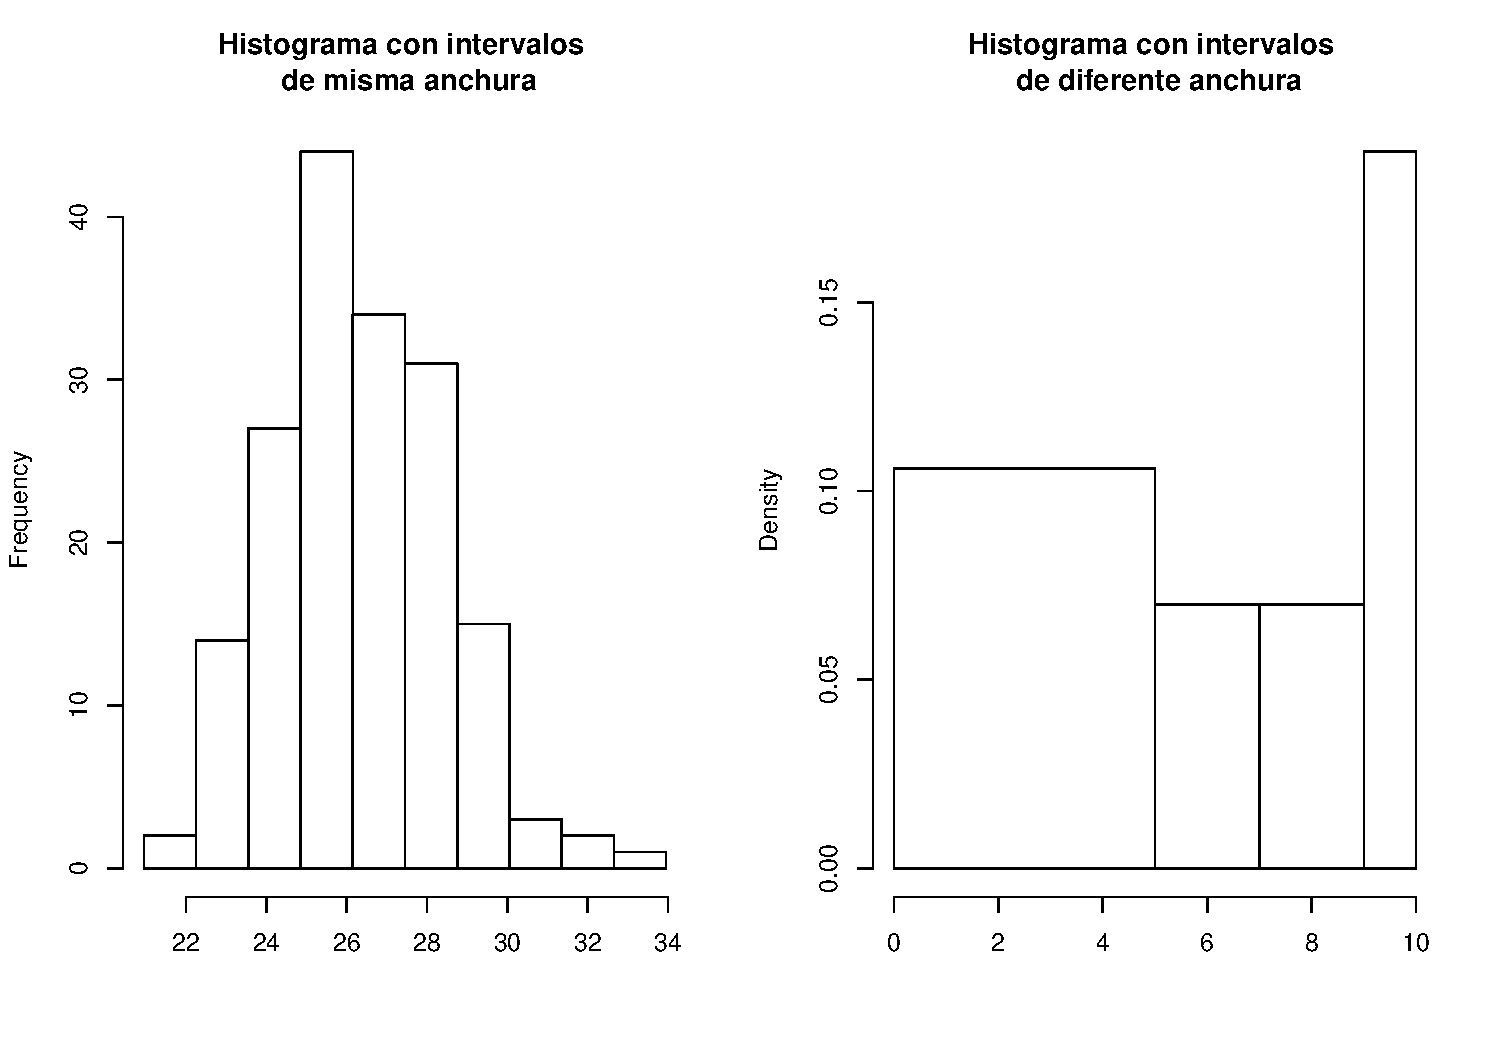
\includegraphics{Tema9.-Agrupacion_datos_cuantitativos_files/figure-beamer/unnamed-chunk-43-1.pdf}

\end{frame}

\begin{frame}{Interpretación de los histogramas}
\protect\hypertarget{interpretaciuxf3n-de-los-histogramas-2}{}

\begin{itemize}
\tightlist
\item
  Histograma de frecuencias relativas: la altura, densidad, de cada
  barra es la necesaria para que el área sea igual a la frecuencia
  relativa de la clase. La suma de todas las áreas debe ser 1. De nuevo,
  conviene indicar de alguna forma la frecuencia que representa cada
  barra.
\item
  Histogramas de frecuencias acumuladas: las alturas de las barras son
  iguales a las frecuencias acumuladas de las clases, independientemente
  de su amplitud.
\end{itemize}

\end{frame}

\begin{frame}{Frecuencias nulas}
\protect\hypertarget{frecuencias-nulas}{}

No es conveniente que en un histograma aparezcan clases con frecuencia
nula, exceptuando el caso en que represente poblaciones muy diferentes y
separadas sin individuos intermedios.

Si apareciesen clases vacías, convendría utilizar un número menor de
clases, o bien unir las clases vacías con alguna de sus adyacentes. De
este último modo romperíamos nuestro modo de trabajar con clases de la
misma amplitud.

\end{frame}

\begin{frame}[fragile]{Dibujando histogramas con R}
\protect\hypertarget{dibujando-histogramas-con-r}{}

Lo hacemos con la función \texttt{hist}, la cual ya conocemos. Su
sintaxis es

\texttt{hist(x,\ breaks=...,\ freq=...,\ right=...,\ ...)}

\begin{itemize}
\tightlist
\item
  \texttt{x}: vector de los datos
\item
  \texttt{breaks}: vector con los extremos de los intervalos o el número
  \(k\) de intervalos. Incluso podemos indicar, entre comillas, el
  método que deseemos para calcular el número de clases:
  \texttt{"Scott"}, \texttt{"Sturges"}\ldots{} Eso sí, para cualquiera
  de las dos últimas opciones, no siempre obtendréis el número deseado
  de intervalos, puesto que R lo considerará solo como sugerencia.
  Además, recordad que el método para calcular los intervalos es
  diferente al de la función \texttt{cut}. Por tanto, se recomienda
  hacer uso de la primera opción.
\item
  \texttt{freq=TRUE}, que es su valor por defecto, produce el histograma
  de frecuencias absolutas si los intervalos son todos de la misma
  amplitud y de frecuencias relativas en caso contrario.
  \texttt{freq=FALSE} nos produce siempre el de frecuencias relativas.
\end{itemize}

\end{frame}

\begin{frame}[fragile]{Dibujando histogramas con R}
\protect\hypertarget{dibujando-histogramas-con-r-1}{}

\begin{itemize}
\tightlist
\item
  \texttt{right} funciona exactamente igual que en la función
  \texttt{cut}.
\item
  \texttt{include.lowest\ =\ TRUE} también funciona exactamente igual
  que en la función \texttt{cut}.
\item
  También podéis utilizar los parámetros de la función \texttt{plot} que
  tengan sentido
\end{itemize}

\texttt{hist} titula por defecto los histogramas del siguiente modo:
``Histogram of'' seguido del nombre del vector de datos. No suele quedar
muy bien si no estamos haciendo nuestro análisis en inglés.

\end{frame}

\begin{frame}[fragile]{Dibujando histogramas con R}
\protect\hypertarget{dibujando-histogramas-con-r-2}{}

Recordemos que el parámetro \texttt{plot} igualado a \texttt{FALSE} no
dibujaba, pero sí calculaba el histograma.

La función \texttt{hist} contiene mucha información en su estructura
interna

\begin{itemize}
\tightlist
\item
  \texttt{breaks} contiene el vector de extremos de los intervalos:
  \(L_1,\dots,L_{k+1}\)
\item
  \texttt{mids} contiene los puntos medios de los intervalos, lo que
  nosotros consideramos las marcas de clase: \(X_1,\dots,X_k\)
\item
  \texttt{counts} contiene el vector de frecuencias absolutas de los
  intervalos: \(n_1,\dots,n_k\)
\item
  \texttt{density} contiene el vector de las densidades de los
  intervalos. Estas se corresponden con las alturas de las barras del
  histograma de frecuencias relativas. Recordemos, la densidad de un
  intervalo es su frecuencia relativa divida por su amplitud.
\end{itemize}

\end{frame}

\begin{frame}[fragile]{Dibujando histogramas con R}
\protect\hypertarget{dibujando-histogramas-con-r-3}{}

Aquí os dejamos una función útil para calcular histogramas de
frecuencias absolutas más completos:

\begin{Shaded}
\begin{Highlighting}[]
\NormalTok{histAbs =}\StringTok{ }\ControlFlowTok{function}\NormalTok{(x,L) \{}
\NormalTok{  h =}\StringTok{ }\KeywordTok{hist}\NormalTok{(x, }\DataTypeTok{breaks =}\NormalTok{ L, }\DataTypeTok{right =} \OtherTok{FALSE}\NormalTok{, }\DataTypeTok{freq =} \OtherTok{FALSE}\NormalTok{,}
           \DataTypeTok{xaxt =} \StringTok{"n"}\NormalTok{, }\DataTypeTok{yaxt =} \StringTok{"n"}\NormalTok{, }\DataTypeTok{col =} \StringTok{"lightgray"}\NormalTok{, }
           \DataTypeTok{main =} \StringTok{"Histograma de frecuencias absolutas"}\NormalTok{, }
           \DataTypeTok{xlab =} \StringTok{"Intervalos y marcas de clase"}\NormalTok{,}\DataTypeTok{ylab =} \StringTok{"Frecuencias absolutas"}\NormalTok{)}
  \KeywordTok{axis}\NormalTok{(}\DecValTok{1}\NormalTok{, }\DataTypeTok{at=}\NormalTok{L)}
  \KeywordTok{text}\NormalTok{(h}\OperatorTok{$}\NormalTok{mids, h}\OperatorTok{$}\NormalTok{density}\OperatorTok{/}\DecValTok{2}\NormalTok{, }\DataTypeTok{labels=}\NormalTok{h}\OperatorTok{$}\NormalTok{counts, }\DataTypeTok{col=}\StringTok{"purple"}\NormalTok{) }
\NormalTok{  \}}
\end{Highlighting}
\end{Shaded}

\begin{itemize}
\tightlist
\item
  \texttt{xaxt="n"} e \texttt{yaxt="n"} especifican que, por ahora, la
  función no dibuje los ejes de abcisas y ordenadas, respectivamente.
\end{itemize}

\end{frame}

\begin{frame}[fragile]{Dibujando histogramas con R}
\protect\hypertarget{dibujando-histogramas-con-r-4}{}

\begin{itemize}
\tightlist
\item
  \texttt{axis(i,\ at=...)} dibuja el eje correspondiente al valor de
  \(i\) con marcas en los lugares indicados por el vector definido
  mediante \texttt{at}. Si \(i=1\), el de abcisas; si \(i=2\), el de
  ordenadas.
\end{itemize}

Os habréis fijado que con \texttt{freq\ =\ FALSE} en realidad hemos
dibujado un histograma de frecuencias relativas, pero al haber omitido
el eje de ordenadas, da lo mismo. En cambio, sí que nos ha sido útil
para poder añadir, con la función \texttt{text}, la frecuencia absoluta
de cada clase sobre el punto medio de su intervalo, los valores
\texttt{h\$mids} y a media algura de su barra, correspondiente a
\texttt{h\$density} gracias a que, con \texttt{freq\ =\ FALSE} estas
alturas se corresponden con la densidad.

\end{frame}

\begin{frame}[fragile]{Dibujando histogramas con R}
\protect\hypertarget{dibujando-histogramas-con-r-5}{}

Otra forma de indicar las frecuencias absolutas de las barras es
utilizar la función \texttt{rug}, la cual permite añadir al histograma
una ``alfombra'' con marcas en todos los valores del vector, donde el
grosor de cada marca es proporcional a la frecuencia del valor que
representa.

Existe la posibilidad de añadir un poco de ruido a los datos de un
vector para deshacer posibles empates. Esto lo conseguimos combinando la
función \texttt{rug} con \texttt{jitter}.

\end{frame}

\begin{frame}{Dibujando histogramas con R}
\protect\hypertarget{dibujando-histogramas-con-r-6}{}

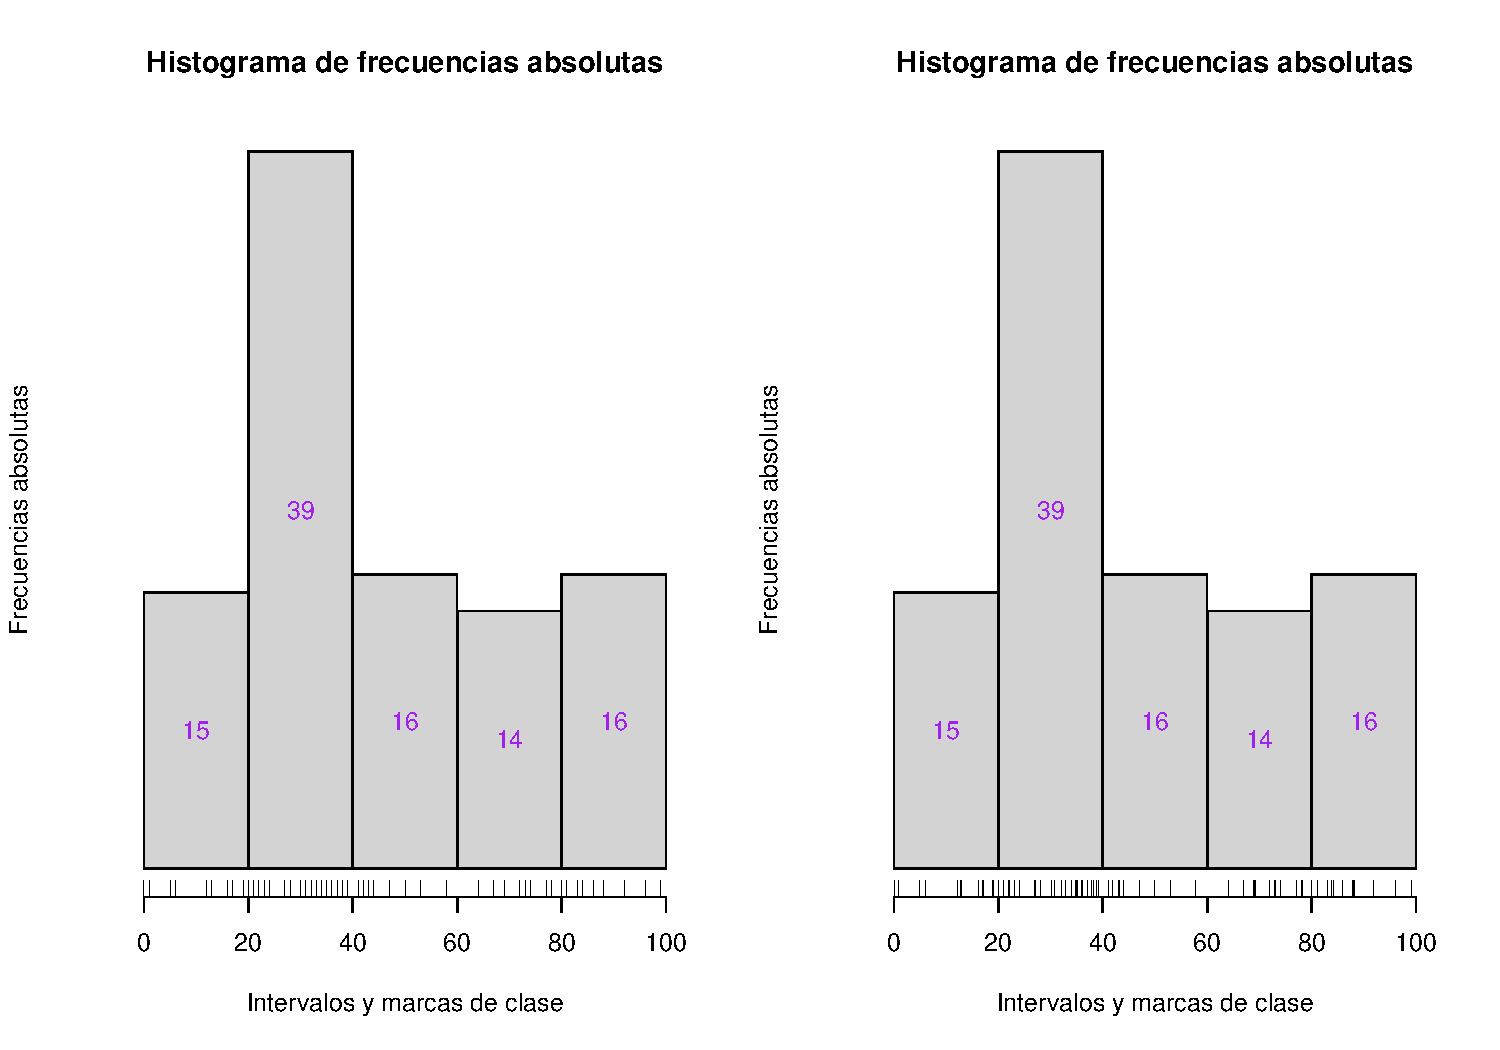
\includegraphics{Tema9.-Agrupacion_datos_cuantitativos_files/figure-beamer/unnamed-chunk-45-1.pdf}

\end{frame}

\begin{frame}[fragile]{Dibujando histogramas con R}
\protect\hypertarget{dibujando-histogramas-con-r-7}{}

Aquí os dejamos una función útil para calcular histogramas de
frecuencias absolutas acumuladas más completos:

\begin{Shaded}
\begin{Highlighting}[]
\NormalTok{histAbsCum =}\StringTok{ }\ControlFlowTok{function}\NormalTok{(x,L) \{}
\NormalTok{  h =}\StringTok{ }\KeywordTok{hist}\NormalTok{(x, }\DataTypeTok{breaks =}\NormalTok{ L, }\DataTypeTok{right =} \OtherTok{FALSE}\NormalTok{ , }\DataTypeTok{plot =} \OtherTok{FALSE}\NormalTok{) }
\NormalTok{  h}\OperatorTok{$}\NormalTok{density =}\StringTok{ }\KeywordTok{cumsum}\NormalTok{(h}\OperatorTok{$}\NormalTok{density)}
  \KeywordTok{plot}\NormalTok{(h, }\DataTypeTok{freq =} \OtherTok{FALSE}\NormalTok{, }\DataTypeTok{xaxt =} \StringTok{"n"}\NormalTok{, }\DataTypeTok{yaxt =} \StringTok{"n"}\NormalTok{, }\DataTypeTok{col =} \StringTok{"lightgray"}\NormalTok{, }
       \DataTypeTok{main =} \StringTok{"Histograma de frecuencias}\CharTok{\textbackslash{}n}\StringTok{absolutas acumuladas"}\NormalTok{, }\DataTypeTok{xlab =} \StringTok{"Intervalos"}\NormalTok{, }
       \DataTypeTok{ylab =} \StringTok{"Frec. absolutas acumuladas"}\NormalTok{)}
  \KeywordTok{axis}\NormalTok{(}\DecValTok{1}\NormalTok{, }\DataTypeTok{at=}\NormalTok{L)}
  \KeywordTok{text}\NormalTok{(h}\OperatorTok{$}\NormalTok{mids, h}\OperatorTok{$}\NormalTok{density}\OperatorTok{/}\DecValTok{2}\NormalTok{, }\DataTypeTok{labels =} \KeywordTok{cumsum}\NormalTok{(h}\OperatorTok{$}\NormalTok{counts), }\DataTypeTok{col =} \StringTok{"purple"}\NormalTok{) }
\NormalTok{  \}}
\end{Highlighting}
\end{Shaded}

\end{frame}

\begin{frame}[fragile]{Dibujando histogramas con R}
\protect\hypertarget{dibujando-histogramas-con-r-8}{}

Con la función anterior, lo que hacemos es, en primer lugar, producir el
histograma básico de los datos, sin dibujarlo para a continuación
modificar la componente \texttt{density} para que contenga las sumas
acumuladas de esta componente del histograma original.

Seguidamente, dibujamos el nuevo histograma resultante, aplicando la
función \texttt{plot}. Es aquí donde debemos especificar los parámetros
y no en el histograma original.

Finalmente, añadimos el eje de abcisas y las frecuencias acumuladas en
color lila.

\end{frame}

\begin{frame}{Dibujando histogramas con R}
\protect\hypertarget{dibujando-histogramas-con-r-9}{}

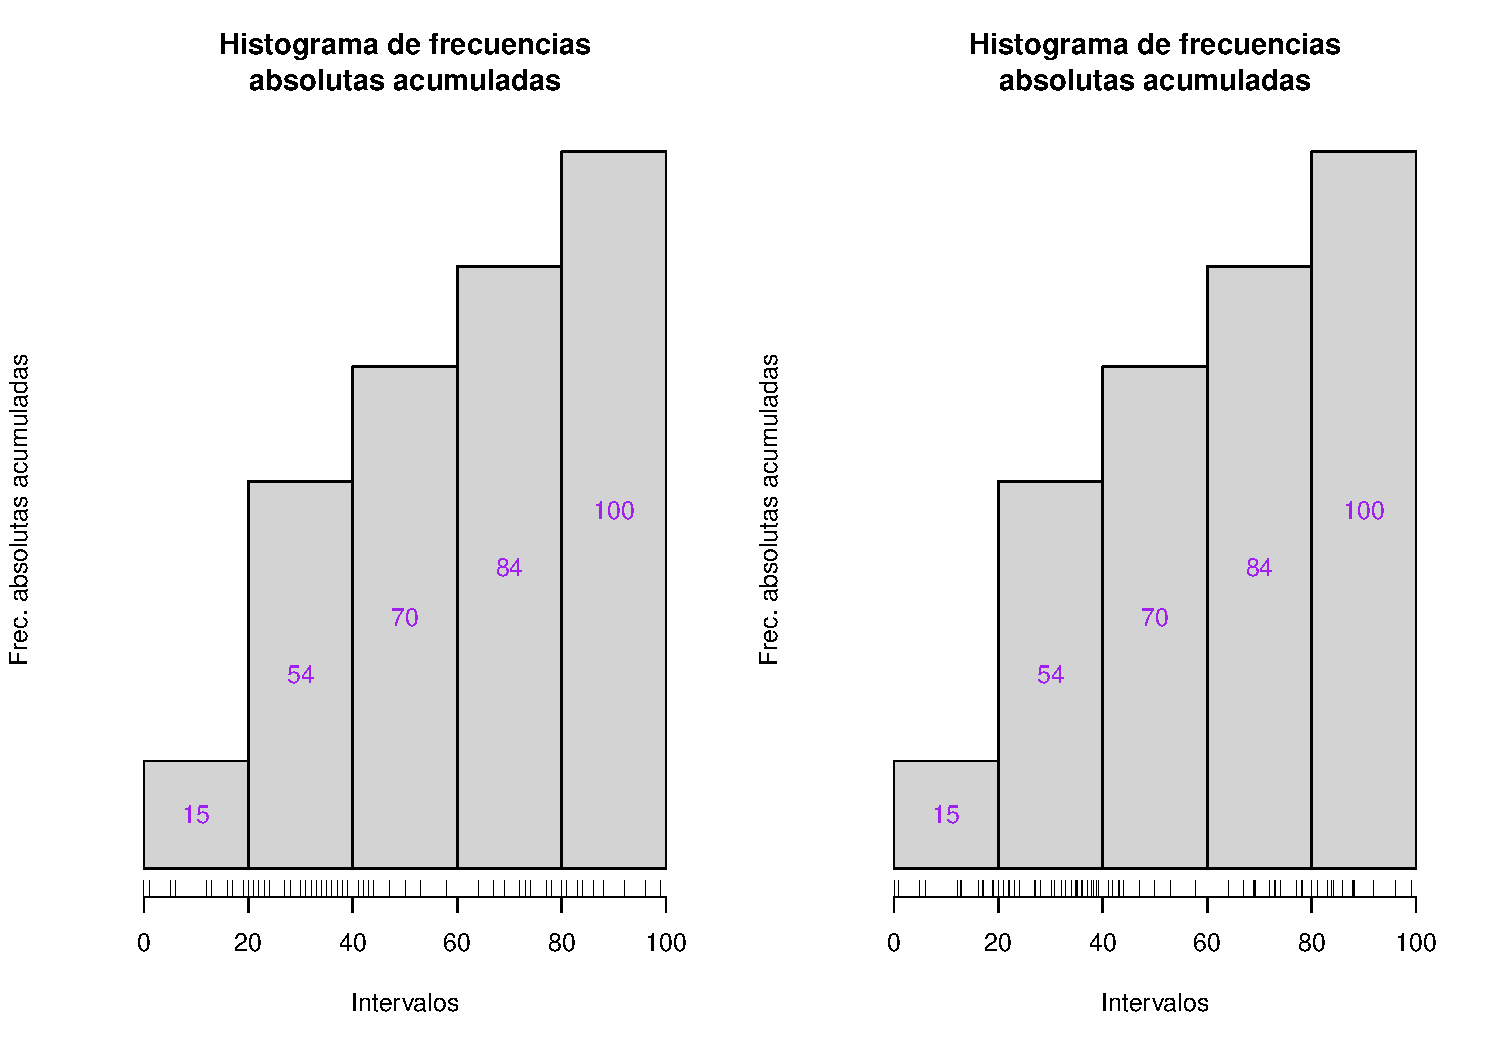
\includegraphics{Tema9.-Agrupacion_datos_cuantitativos_files/figure-beamer/unnamed-chunk-47-1.pdf}

\end{frame}

\begin{frame}{Histogramas de frecuencias relativas}
\protect\hypertarget{histogramas-de-frecuencias-relativas}{}

En estos histogramas, es común superponer una curva que estime la
densidad de la distribución de la variable cuantitativa definida por la
característica que estamos midiendo.

La densidad de una variable es una curva cuya área comprendida entre el
eje de las abcisas y la propia curva sobre un intervalo es igual a la
fracción de individuos de la población que caen dentro de ese intervalo.

Para hacernos una idea visual, imaginad que vais aumentando el tamaño de
la muestra a la vez que agrupáis los datos en un conjunto cada vez mayor
de clases. Si el rango de los datos se mantiene constante, la amplitud
de las clases del histograma irá menguando. Además, cuando \(n\), el
tamaño de la muestra, tiende a infinito, los intervalos tienden a ser
puntos y, a su vez, las barras tienden a ser líneas verticales. Pues
bien, los extremos superiores de estas líneas serán los que dibujen la
densidad de la variable.

\end{frame}

\begin{frame}{Campana de Gauss}
\protect\hypertarget{campana-de-gauss}{}

Es la densidad más famosa: la
\href{https://es.wikipedia.org/wiki/Función_gaussiana}{Campana de Gauss}
Ésta se corresponde con una variable que siga una distribución nomal.

La forma de la campana depende de dos parámetros: el valor medio,
\(\mu\), y su desviación típica, \(\sigma\).

\begin{figure}
\centering
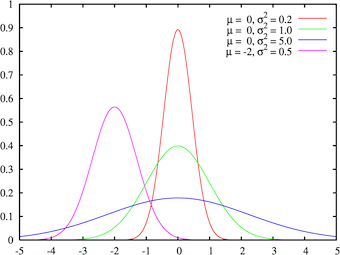
\includegraphics{Imgs/gauss.png}
\caption{Campana de Gauss en función de diferentes valores de \(\mu\) y
\(\sigma\)}
\end{figure}

\end{frame}

\begin{frame}[fragile]{Dibujando la curva de densidad}
\protect\hypertarget{dibujando-la-curva-de-densidad}{}

Existen muchos métodos con los cuales estimar la densidad de
distribución a partir de una muestra.

Una de ellas es mediante la función \texttt{density} de R. Al aplicarla
a un conjunto de datos, produce una \texttt{list} que incluye los
vectores \texttt{x} e \texttt{y} que continen la primera y segunda
coordenadas, respectivamente, de 512 puntos de la forma \((x,y)\) sobre
la curva de densidad estimada.

Aplicando \texttt{plot} o \texttt{lines} a este resultado según
pertoque, obtenemos la representación gráfica de esta curva.

\end{frame}

\begin{frame}[fragile]{Histogramas de frecuencias relativas}
\protect\hypertarget{histogramas-de-frecuencias-relativas-1}{}

Aquí os dejamos una función útil para calcular histogramas de
frecuencias relativas más completos:

\begin{Shaded}
\begin{Highlighting}[]
\NormalTok{histRel =}\StringTok{ }\ControlFlowTok{function}\NormalTok{(x,L) \{}
\NormalTok{  h =}\StringTok{ }\KeywordTok{hist}\NormalTok{(x, }\DataTypeTok{breaks=}\NormalTok{L, }\DataTypeTok{right=}\OtherTok{FALSE}\NormalTok{ , }\DataTypeTok{plot=}\OtherTok{FALSE}\NormalTok{)}
\NormalTok{  t =}\StringTok{ }\KeywordTok{round}\NormalTok{(}\FloatTok{1.1}\OperatorTok{*}\KeywordTok{max}\NormalTok{(}\KeywordTok{max}\NormalTok{(}\KeywordTok{density}\NormalTok{(x)[[}\DecValTok{2}\NormalTok{]]),h}\OperatorTok{$}\NormalTok{density),}\DecValTok{2}\NormalTok{) }
  \KeywordTok{plot}\NormalTok{(h, }\DataTypeTok{freq =} \OtherTok{FALSE}\NormalTok{, }\DataTypeTok{col =} \StringTok{"lightgray"}\NormalTok{, }
       \DataTypeTok{main =} \StringTok{"Histograma de frec. relativas}\CharTok{\textbackslash{}n}\StringTok{y curva de densidad estimada"}\NormalTok{, }
       \DataTypeTok{xaxt=}\StringTok{"n"}\NormalTok{, }\DataTypeTok{ylim=}\KeywordTok{c}\NormalTok{(}\DecValTok{0}\NormalTok{,t), }\DataTypeTok{xlab=}\StringTok{"Intervalos"}\NormalTok{, }\DataTypeTok{ylab=}\StringTok{"Densidades"}\NormalTok{)}
  \KeywordTok{axis}\NormalTok{(}\DecValTok{1}\NormalTok{, }\DataTypeTok{at =}\NormalTok{ L) }
  \KeywordTok{text}\NormalTok{(h}\OperatorTok{$}\NormalTok{mids, h}\OperatorTok{$}\NormalTok{density}\OperatorTok{/}\DecValTok{2}\NormalTok{, }\DataTypeTok{labels =} \KeywordTok{round}\NormalTok{(h}\OperatorTok{$}\NormalTok{counts}\OperatorTok{/}\KeywordTok{length}\NormalTok{(x),}\DecValTok{2}\NormalTok{), }\DataTypeTok{col =} \StringTok{"blue"}\NormalTok{)}
  \KeywordTok{lines}\NormalTok{(}\KeywordTok{density}\NormalTok{(x), }\DataTypeTok{col =} \StringTok{"purple"}\NormalTok{, }\DataTypeTok{lwd =} \DecValTok{2}\NormalTok{) }
\NormalTok{  \}}
\end{Highlighting}
\end{Shaded}

\end{frame}

\begin{frame}{Histogramas de frecuencias relativas}
\protect\hypertarget{histogramas-de-frecuencias-relativas-2}{}

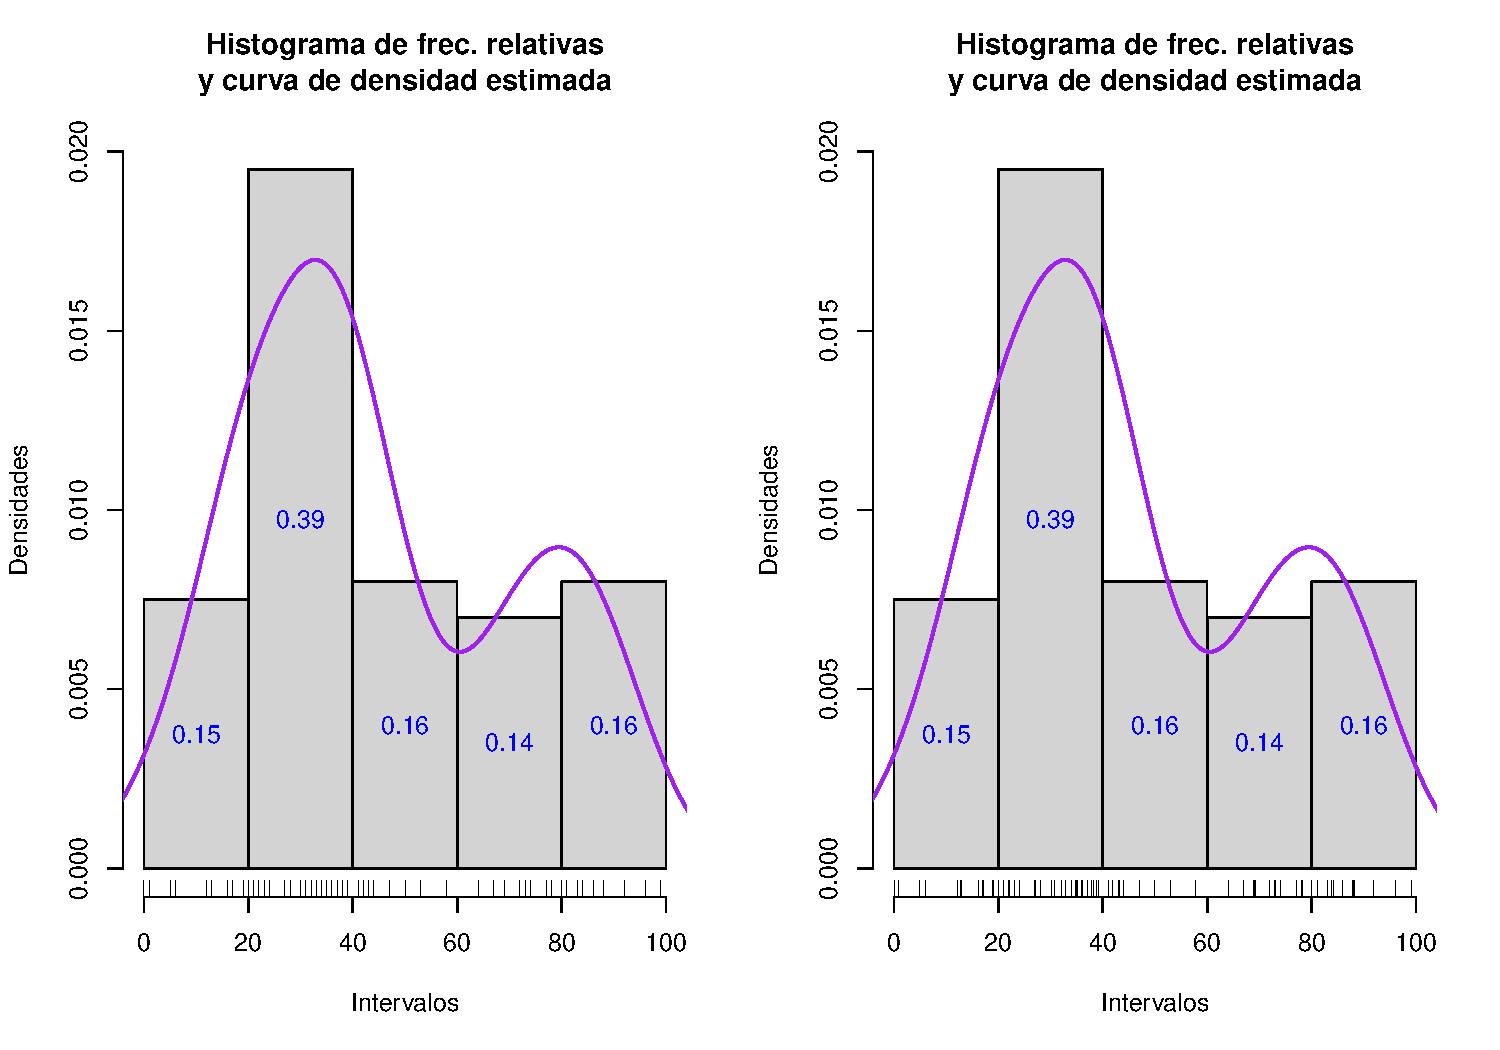
\includegraphics{Tema9.-Agrupacion_datos_cuantitativos_files/figure-beamer/unnamed-chunk-49-1.pdf}

\end{frame}

\begin{frame}{Histogramas de frecuencias relativas acumuladas}
\protect\hypertarget{histogramas-de-frecuencias-relativas-acumuladas}{}

En este último tipo de histograma, se suele superponer una curva que
estime la función de distribución de la variable definida por la
característica que estamos midiendo.

Esta función de distribución, en cada punto nos da la fracción de
individuos de la población que caen a la izquierda de este punto: su
frecuencia relativa acumulada.

En general, la función de distribución en un valor determinado se
obtiene hallando el área de la función de densidad que hay a la
izquierda del valor.

\end{frame}

\begin{frame}[fragile]{Histogramas de frecuencias relativas acumuladas}
\protect\hypertarget{histogramas-de-frecuencias-relativas-acumuladas-1}{}

Aquí os dejamos una función útil para calcular histogramas de
frecuencias relativas acumuladas más completos:

\begin{Shaded}
\begin{Highlighting}[]
\NormalTok{histRelCum =}\StringTok{ }\ControlFlowTok{function}\NormalTok{(x,L)\{}
\NormalTok{  h =}\StringTok{ }\KeywordTok{hist}\NormalTok{(x, }\DataTypeTok{breaks =}\NormalTok{ L, }\DataTypeTok{right =} \OtherTok{FALSE}\NormalTok{ , }\DataTypeTok{plot =} \OtherTok{FALSE}\NormalTok{)}
\NormalTok{  h}\OperatorTok{$}\NormalTok{density =}\StringTok{ }\KeywordTok{cumsum}\NormalTok{(h}\OperatorTok{$}\NormalTok{counts)}\OperatorTok{/}\KeywordTok{length}\NormalTok{(x)}
  \KeywordTok{plot}\NormalTok{(h, }\DataTypeTok{freq =} \OtherTok{FALSE}\NormalTok{, }
      \DataTypeTok{main =} \StringTok{"Histograma de frec. rel. acumuladas}\CharTok{\textbackslash{}n}\StringTok{ y curva de distribución estimada"}\NormalTok{, }
      \DataTypeTok{xaxt =} \StringTok{"n"}\NormalTok{, }\DataTypeTok{col =} \StringTok{"lightgray"}\NormalTok{, }\DataTypeTok{xlab =} \StringTok{"Intervalos"}\NormalTok{, }
      \DataTypeTok{ylab =} \StringTok{"Frec. relativas acumuladas"}\NormalTok{) }
  \KeywordTok{axis}\NormalTok{(}\DecValTok{1}\NormalTok{, }\DataTypeTok{at =}\NormalTok{ L)}
  \KeywordTok{text}\NormalTok{(h}\OperatorTok{$}\NormalTok{mids, h}\OperatorTok{$}\NormalTok{density}\OperatorTok{/}\DecValTok{2}\NormalTok{, }\DataTypeTok{labels =} \KeywordTok{round}\NormalTok{(h}\OperatorTok{$}\NormalTok{density ,}\DecValTok{2}\NormalTok{), }\DataTypeTok{col =} \StringTok{"blue"}\NormalTok{)}
\NormalTok{  dens.x =}\StringTok{ }\KeywordTok{density}\NormalTok{(x)}
\NormalTok{  dens.x}\OperatorTok{$}\NormalTok{y =}\StringTok{ }\KeywordTok{cumsum}\NormalTok{(dens.x}\OperatorTok{$}\NormalTok{y)}\OperatorTok{*}\NormalTok{(dens.x}\OperatorTok{$}\NormalTok{x[}\DecValTok{2}\NormalTok{]}\OperatorTok{-}\NormalTok{dens.x}\OperatorTok{$}\NormalTok{x[}\DecValTok{1}\NormalTok{]) }
  \KeywordTok{lines}\NormalTok{(dens.x,}\DataTypeTok{col =} \StringTok{"purple"}\NormalTok{,}\DataTypeTok{lwd =} \DecValTok{2}\NormalTok{)}
\NormalTok{\}}
\end{Highlighting}
\end{Shaded}

\end{frame}

\begin{frame}{Histogramas de frecuencias relativas acumuladas}
\protect\hypertarget{histogramas-de-frecuencias-relativas-acumuladas-2}{}

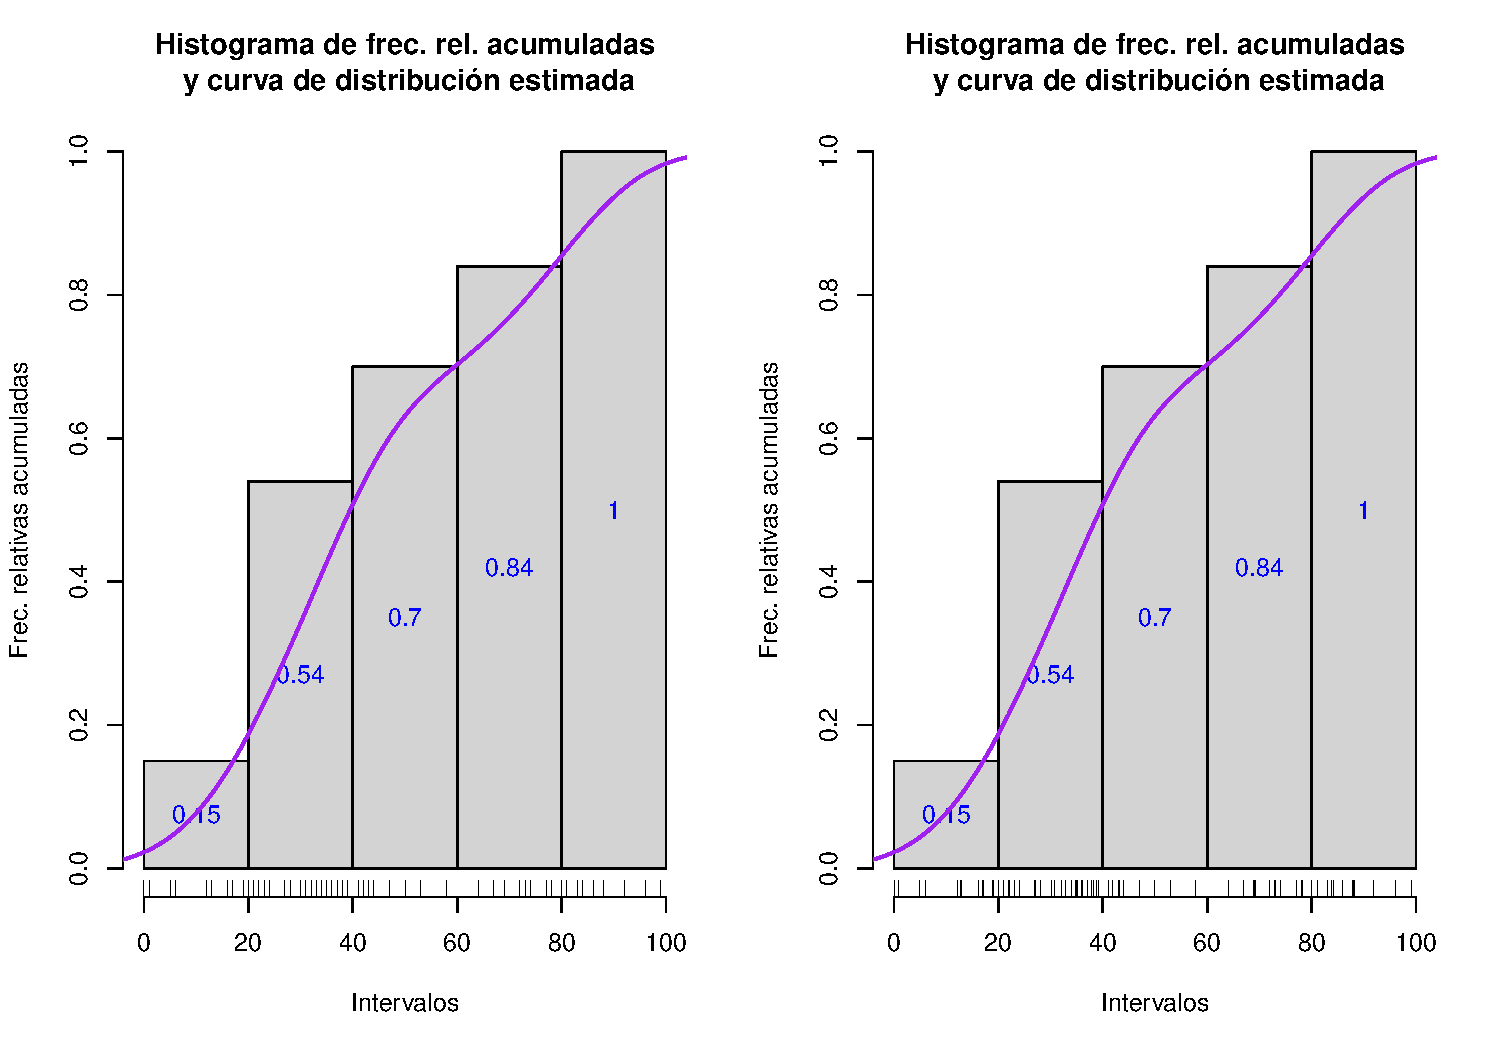
\includegraphics{Tema9.-Agrupacion_datos_cuantitativos_files/figure-beamer/unnamed-chunk-51-1.pdf}

\end{frame}

\hypertarget{ejemplo-2---continuaciuxf3n-1}{%
\section{Ejemplo 2 - Continuación}\label{ejemplo-2---continuaciuxf3n-1}}

\begin{frame}[fragile]{Enunciado}
\protect\hypertarget{enunciado-4}{}

Vamos a seguir trabajando con nuestra variable \texttt{cw} y, esta vez,
lo que haremos será calcular histogramas de todas las formas explicadas
anteriormente.

\end{frame}

\begin{frame}[fragile]{Solución}
\protect\hypertarget{soluciuxf3n-37}{}

Dibujamos el histograma con \texttt{hist} y luego observamos su
información interna.

\begin{Shaded}
\begin{Highlighting}[]
\KeywordTok{hist}\NormalTok{(cw, }\DataTypeTok{breaks =}\NormalTok{ L, }\DataTypeTok{right =} \OtherTok{FALSE}\NormalTok{, }\DataTypeTok{main =} \StringTok{"Histograma de las anchuras de los cangrejos"}\NormalTok{)}
\end{Highlighting}
\end{Shaded}

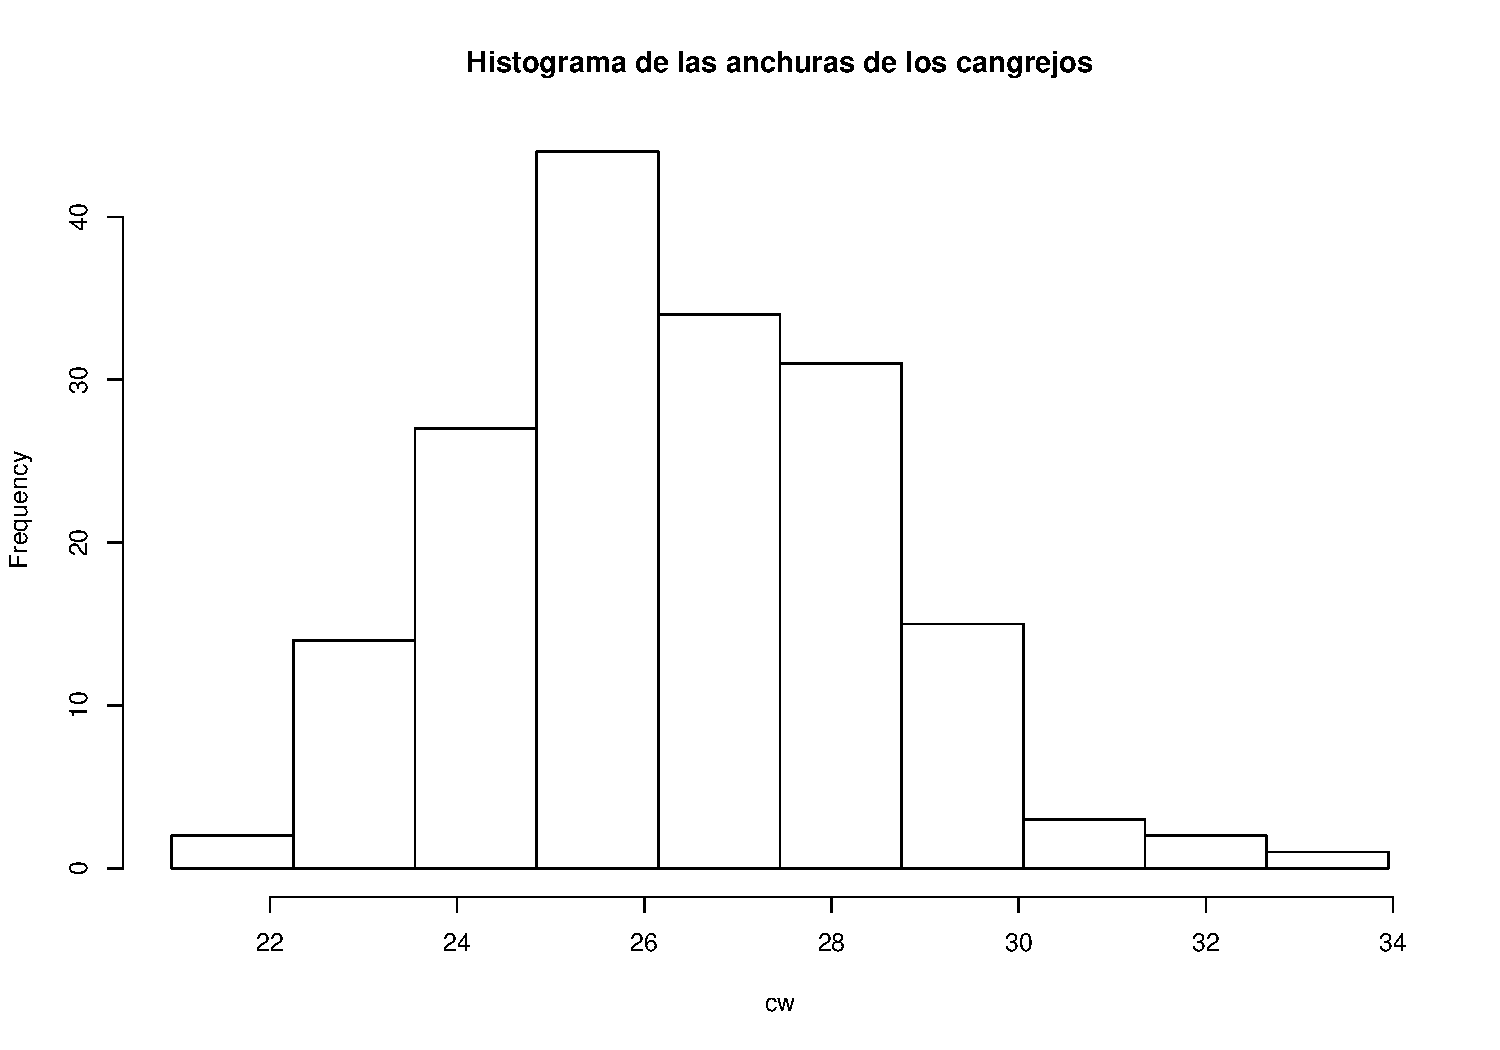
\includegraphics{Tema9.-Agrupacion_datos_cuantitativos_files/figure-beamer/unnamed-chunk-52-1.pdf}

\end{frame}

\begin{frame}[fragile]{Solución}
\protect\hypertarget{soluciuxf3n-38}{}

\begin{Shaded}
\begin{Highlighting}[]
\KeywordTok{hist}\NormalTok{(cw, }\DataTypeTok{breaks =}\NormalTok{ L, }\DataTypeTok{right =} \OtherTok{FALSE}\NormalTok{, }\DataTypeTok{plot =} \OtherTok{FALSE}\NormalTok{)}
\end{Highlighting}
\end{Shaded}

\begin{verbatim}
$breaks
 [1] 20.95 22.25 23.55 24.85 26.15 27.45 28.75 30.05 31.35 32.65 33.95

$counts
 [1]  2 14 27 44 34 31 15  3  2  1

$density
 [1] 0.008892841 0.062249889 0.120053357 0.195642508 0.151178301 0.137839040
 [7] 0.066696309 0.013339262 0.008892841 0.004446421

$mids
 [1] 21.6 22.9 24.2 25.5 26.8 28.1 29.4 30.7 32.0 33.3

$xname
[1] "cw"

$equidist
[1] TRUE

attr(,"class")
[1] "histogram"
\end{verbatim}

\end{frame}

\begin{frame}[fragile]{Solución}
\protect\hypertarget{soluciuxf3n-39}{}

Dibujamos el histograma con \texttt{histAbs}.

\begin{Shaded}
\begin{Highlighting}[]
\KeywordTok{histAbs}\NormalTok{(cw,L)}
\end{Highlighting}
\end{Shaded}

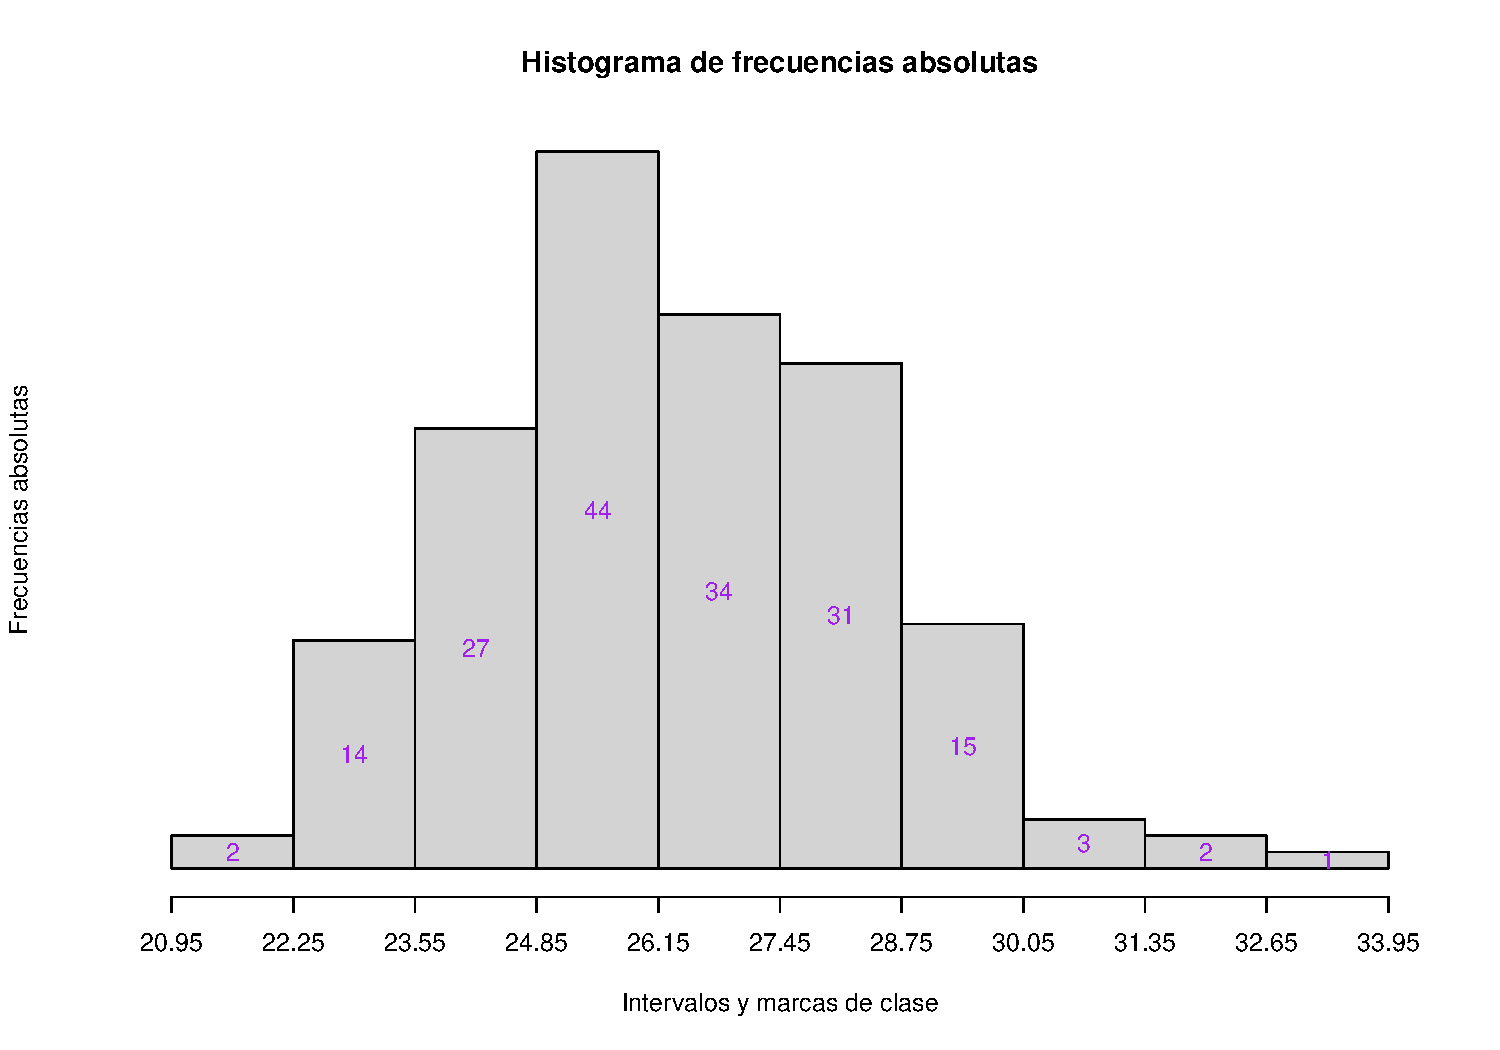
\includegraphics{Tema9.-Agrupacion_datos_cuantitativos_files/figure-beamer/unnamed-chunk-54-1.pdf}

\end{frame}

\begin{frame}[fragile]{Solución}
\protect\hypertarget{soluciuxf3n-40}{}

Dibujamos el histograma con \texttt{histAbsCum}.

\begin{Shaded}
\begin{Highlighting}[]
\KeywordTok{histAbsCum}\NormalTok{(cw,L)}
\end{Highlighting}
\end{Shaded}

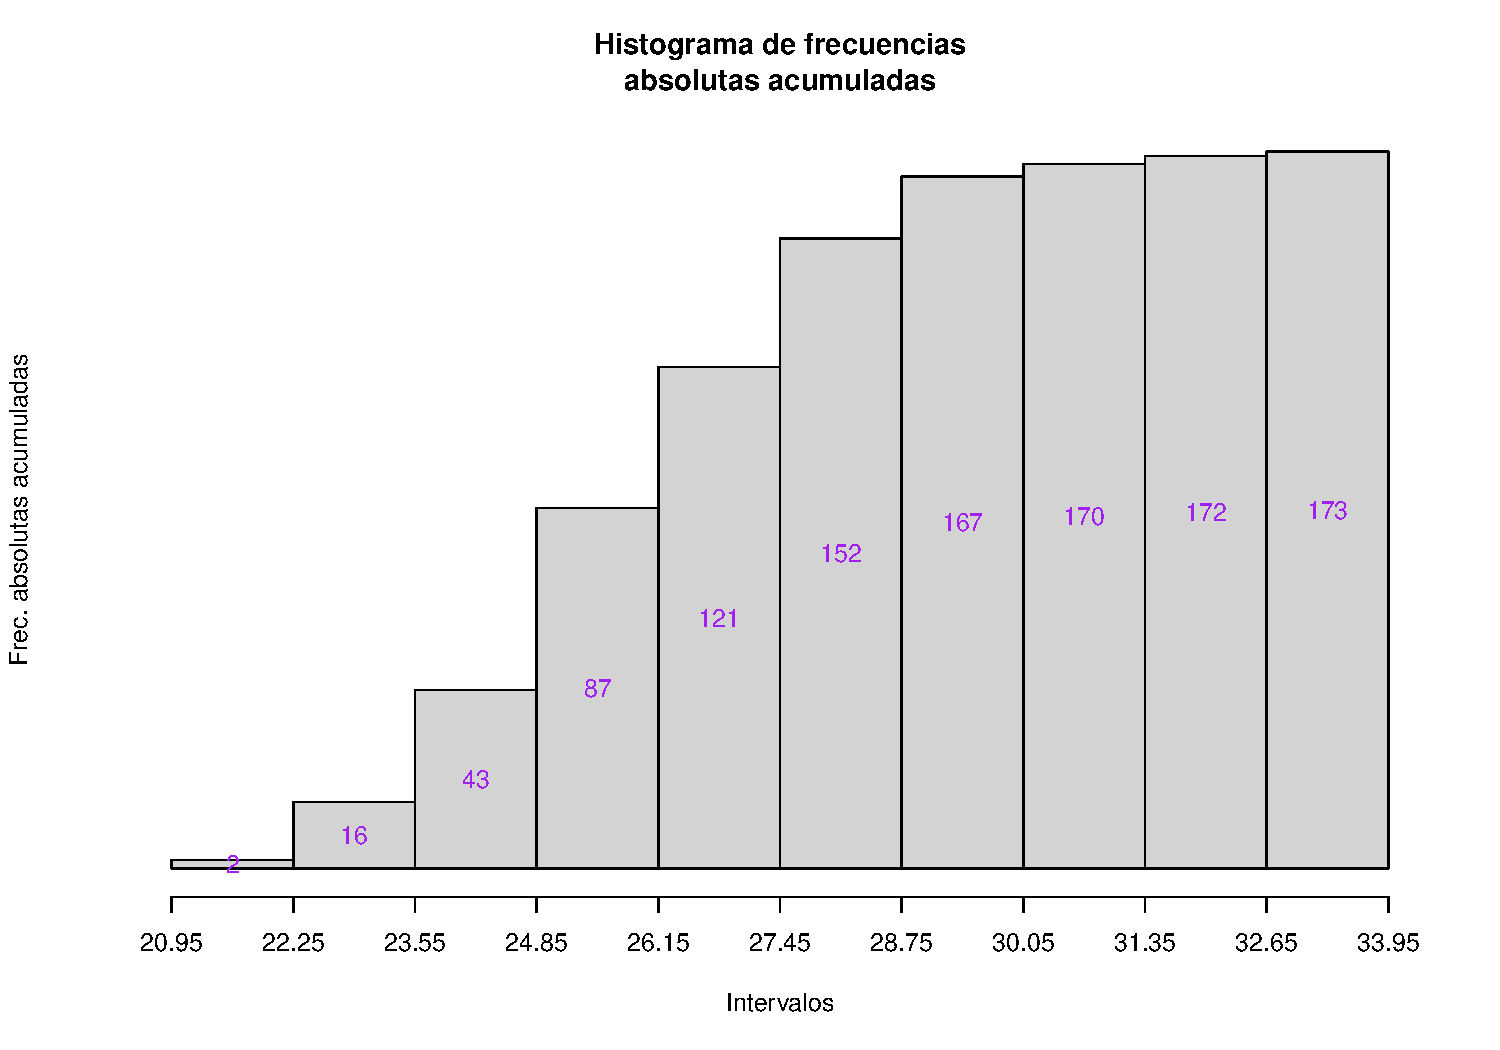
\includegraphics{Tema9.-Agrupacion_datos_cuantitativos_files/figure-beamer/unnamed-chunk-55-1.pdf}

\end{frame}

\begin{frame}[fragile]{Solución}
\protect\hypertarget{soluciuxf3n-41}{}

Hacemos uso de las funciones \texttt{rug} y \texttt{jitter}

\begin{Shaded}
\begin{Highlighting}[]
\KeywordTok{histAbs}\NormalTok{(cw,L)}
\KeywordTok{rug}\NormalTok{(cw)}
\end{Highlighting}
\end{Shaded}

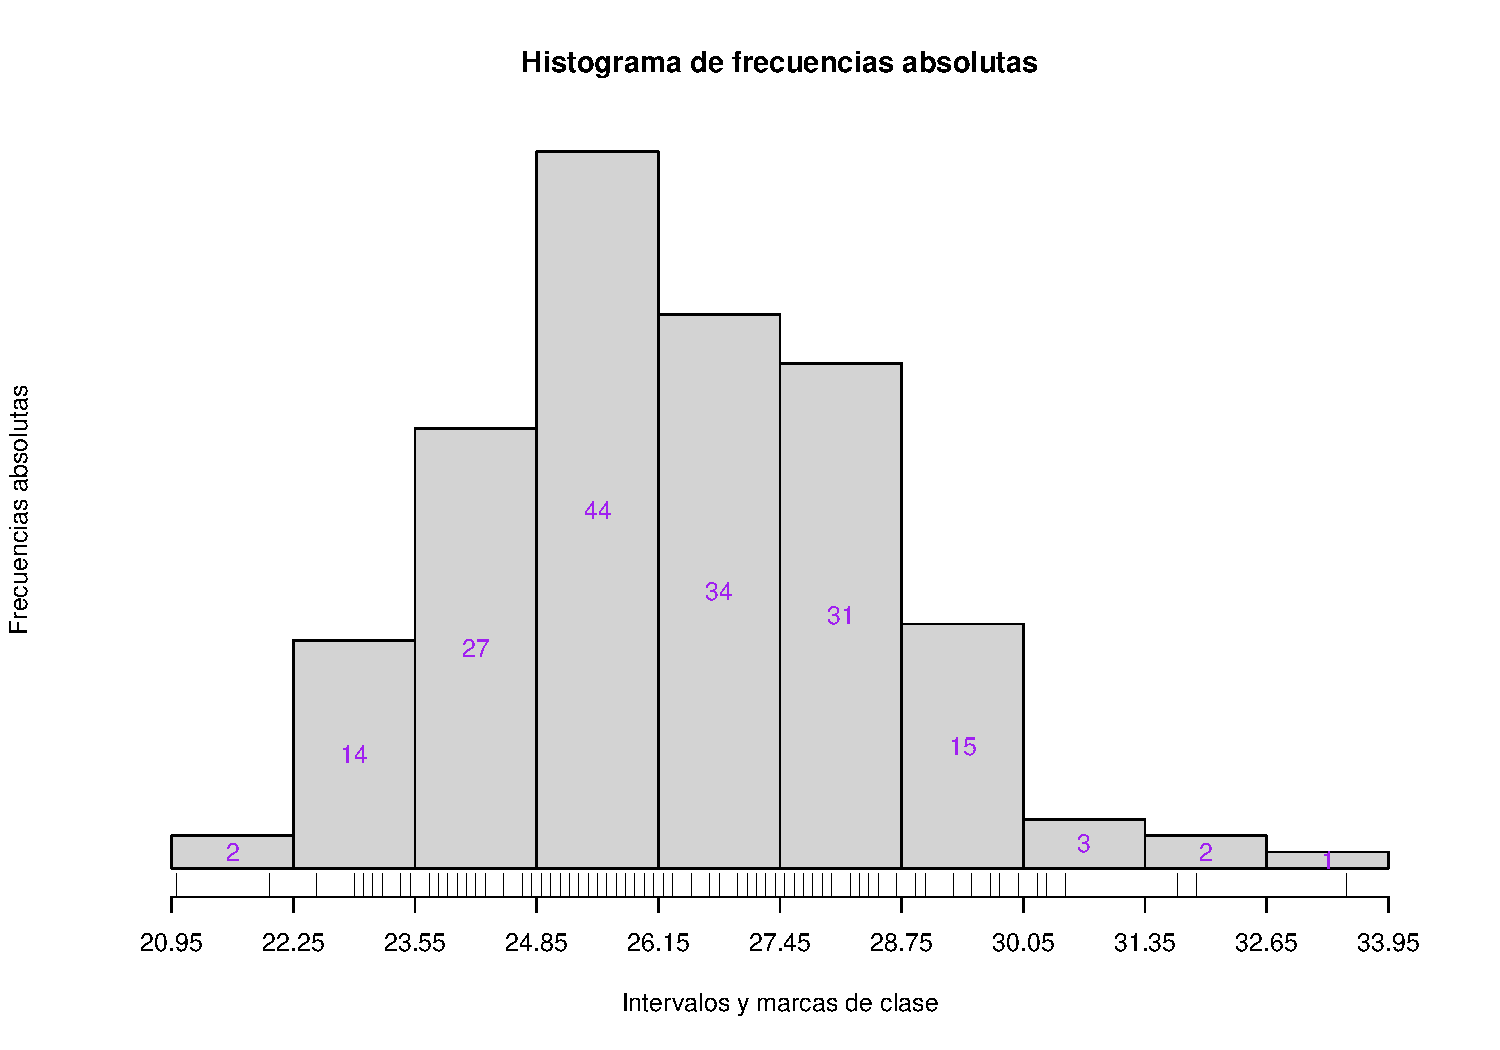
\includegraphics{Tema9.-Agrupacion_datos_cuantitativos_files/figure-beamer/unnamed-chunk-56-1.pdf}

\end{frame}

\begin{frame}[fragile]{Solución}
\protect\hypertarget{soluciuxf3n-42}{}

\begin{Shaded}
\begin{Highlighting}[]
\KeywordTok{histAbs}\NormalTok{(cw,L)}
\KeywordTok{rug}\NormalTok{(}\KeywordTok{jitter}\NormalTok{(cw))}
\end{Highlighting}
\end{Shaded}

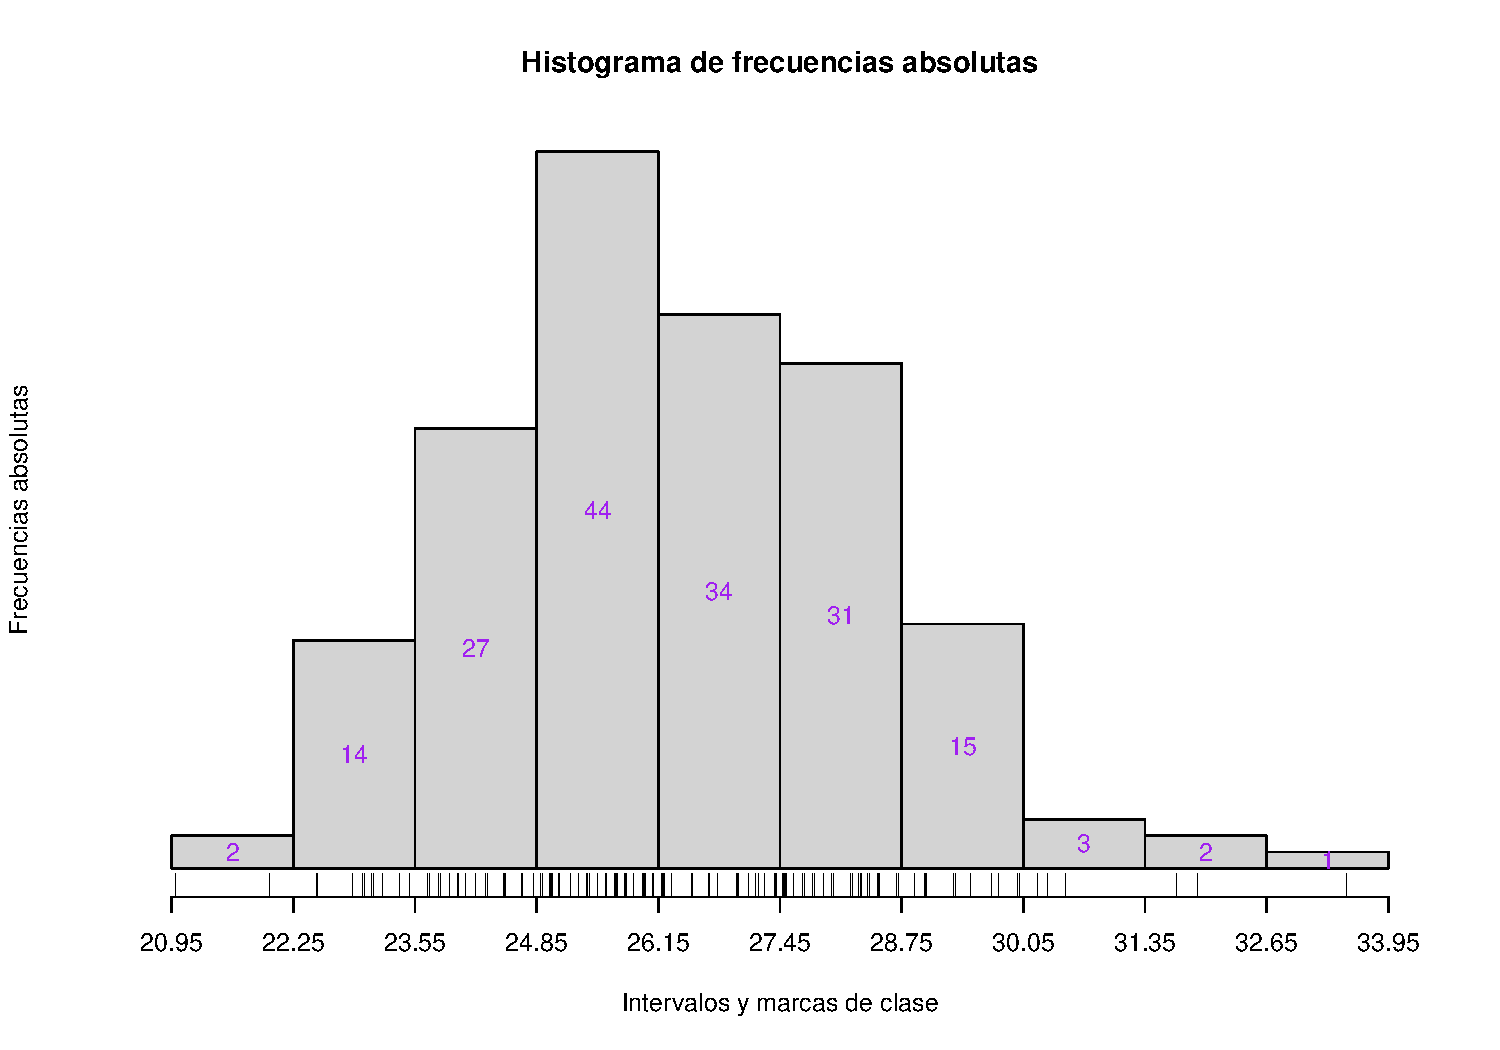
\includegraphics{Tema9.-Agrupacion_datos_cuantitativos_files/figure-beamer/unnamed-chunk-57-1.pdf}

\end{frame}

\begin{frame}[fragile]{Solución}
\protect\hypertarget{soluciuxf3n-43}{}

A continuación, calculamos la densidad de \texttt{cw} y la representamos
con \texttt{histRel}

\begin{Shaded}
\begin{Highlighting}[]
\KeywordTok{str}\NormalTok{(}\KeywordTok{density}\NormalTok{(cw))}
\end{Highlighting}
\end{Shaded}

\begin{verbatim}
List of 7
 $ x        : num [1:512] 19 19 19.1 19.1 19.1 ...
 $ y        : num [1:512] 3.90e-05 4.50e-05 5.17e-05 5.94e-05 6.82e-05 ...
 $ bw       : num 0.671
 $ n        : int 173
 $ call     : language density.default(x = cw)
 $ data.name: chr "cw"
 $ has.na   : logi FALSE
 - attr(*, "class")= chr "density"
\end{verbatim}

\end{frame}

\begin{frame}[fragile]{Solución}
\protect\hypertarget{soluciuxf3n-44}{}

\begin{Shaded}
\begin{Highlighting}[]
\KeywordTok{histRel}\NormalTok{(cw,L)}
\end{Highlighting}
\end{Shaded}

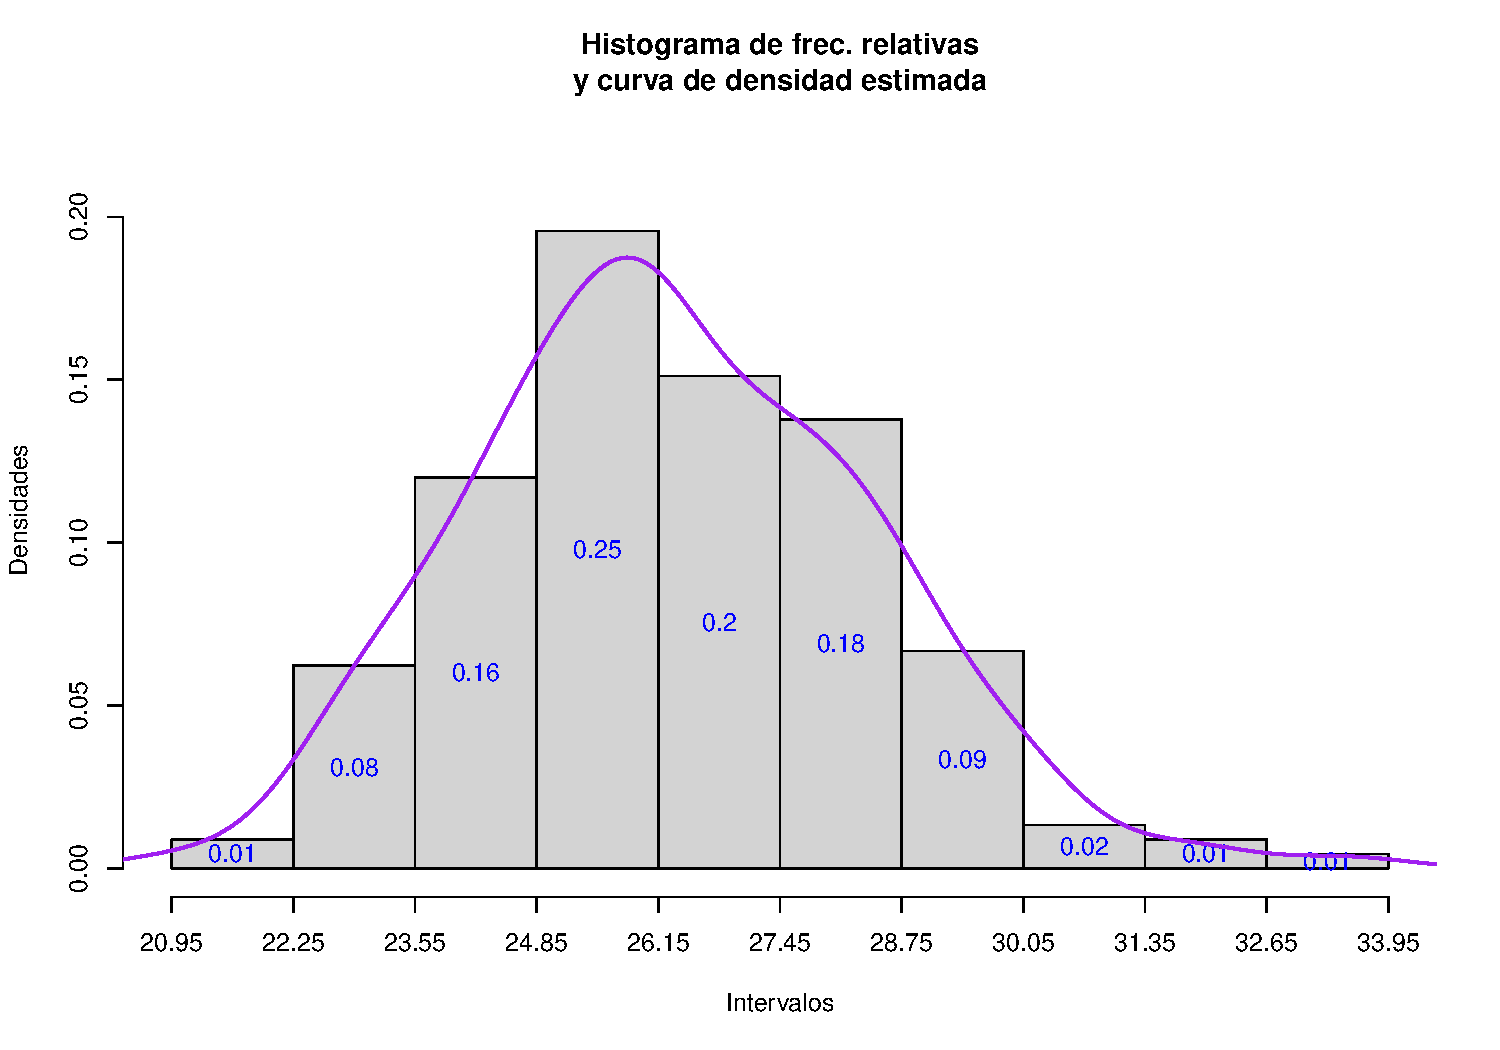
\includegraphics{Tema9.-Agrupacion_datos_cuantitativos_files/figure-beamer/unnamed-chunk-59-1.pdf}

\end{frame}

\begin{frame}[fragile]{Solución}
\protect\hypertarget{soluciuxf3n-45}{}

La curva de densidad que hemos obtenemos en este gráfico tiene una forma
de campana que nos recuerda la campana de Gauss. Para explorar este
parecido, vamos a añadir al histograma la gráfica de la función densidad
de una distribución normal de media y desviación típica las del conjunto
de datos original

Así, aplicando las instrucciones siguientes, acabamos obteniendo

\begin{Shaded}
\begin{Highlighting}[]
\KeywordTok{histRel}\NormalTok{(cw,L)}
\KeywordTok{curve}\NormalTok{(}\KeywordTok{dnorm}\NormalTok{(x, }\KeywordTok{mean}\NormalTok{(cw), }\KeywordTok{sd}\NormalTok{(cw)), }\DataTypeTok{col=}\StringTok{"cyan4"}\NormalTok{, }\DataTypeTok{lty=}\DecValTok{4}\NormalTok{, }\DataTypeTok{lwd=}\DecValTok{2}\NormalTok{,}
\DataTypeTok{add=}\OtherTok{TRUE}\NormalTok{)}
\KeywordTok{legend}\NormalTok{(}\StringTok{"topright"}\NormalTok{, }\DataTypeTok{lwd=}\KeywordTok{c}\NormalTok{(}\DecValTok{2}\NormalTok{,}\DecValTok{2}\NormalTok{), }\DataTypeTok{lty=}\KeywordTok{c}\NormalTok{(}\DecValTok{1}\NormalTok{,}\DecValTok{4}\NormalTok{), }\DataTypeTok{col=}\KeywordTok{c}\NormalTok{(}\StringTok{"purple"}\NormalTok{,}\StringTok{"cyan4"}\NormalTok{),}
       \DataTypeTok{legend=}\KeywordTok{c}\NormalTok{(}\StringTok{"densidad estimada"}\NormalTok{,}\StringTok{"densidad normal"}\NormalTok{))}
\end{Highlighting}
\end{Shaded}

\end{frame}

\begin{frame}{Solución}
\protect\hypertarget{soluciuxf3n-46}{}

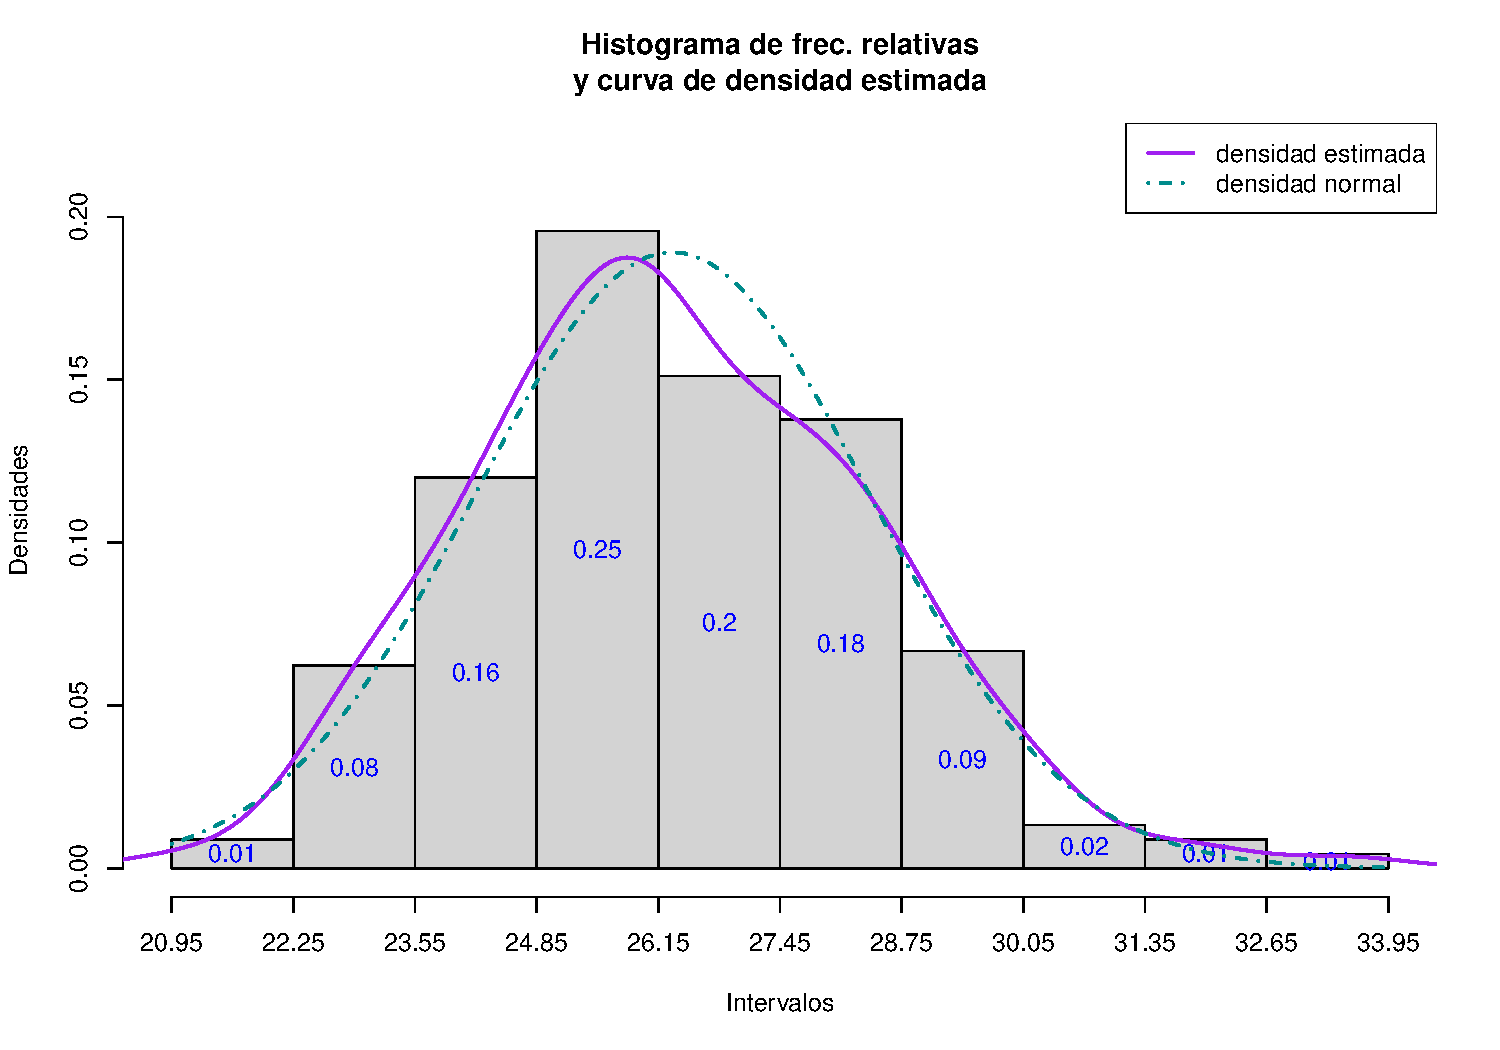
\includegraphics{Tema9.-Agrupacion_datos_cuantitativos_files/figure-beamer/unnamed-chunk-61-1.pdf}

\end{frame}

\begin{frame}[fragile]{Solución}
\protect\hypertarget{soluciuxf3n-47}{}

Dibujamos el histograma con \texttt{histRelCum}.

\begin{Shaded}
\begin{Highlighting}[]
\KeywordTok{histRelCum}\NormalTok{(cw,L)}
\end{Highlighting}
\end{Shaded}

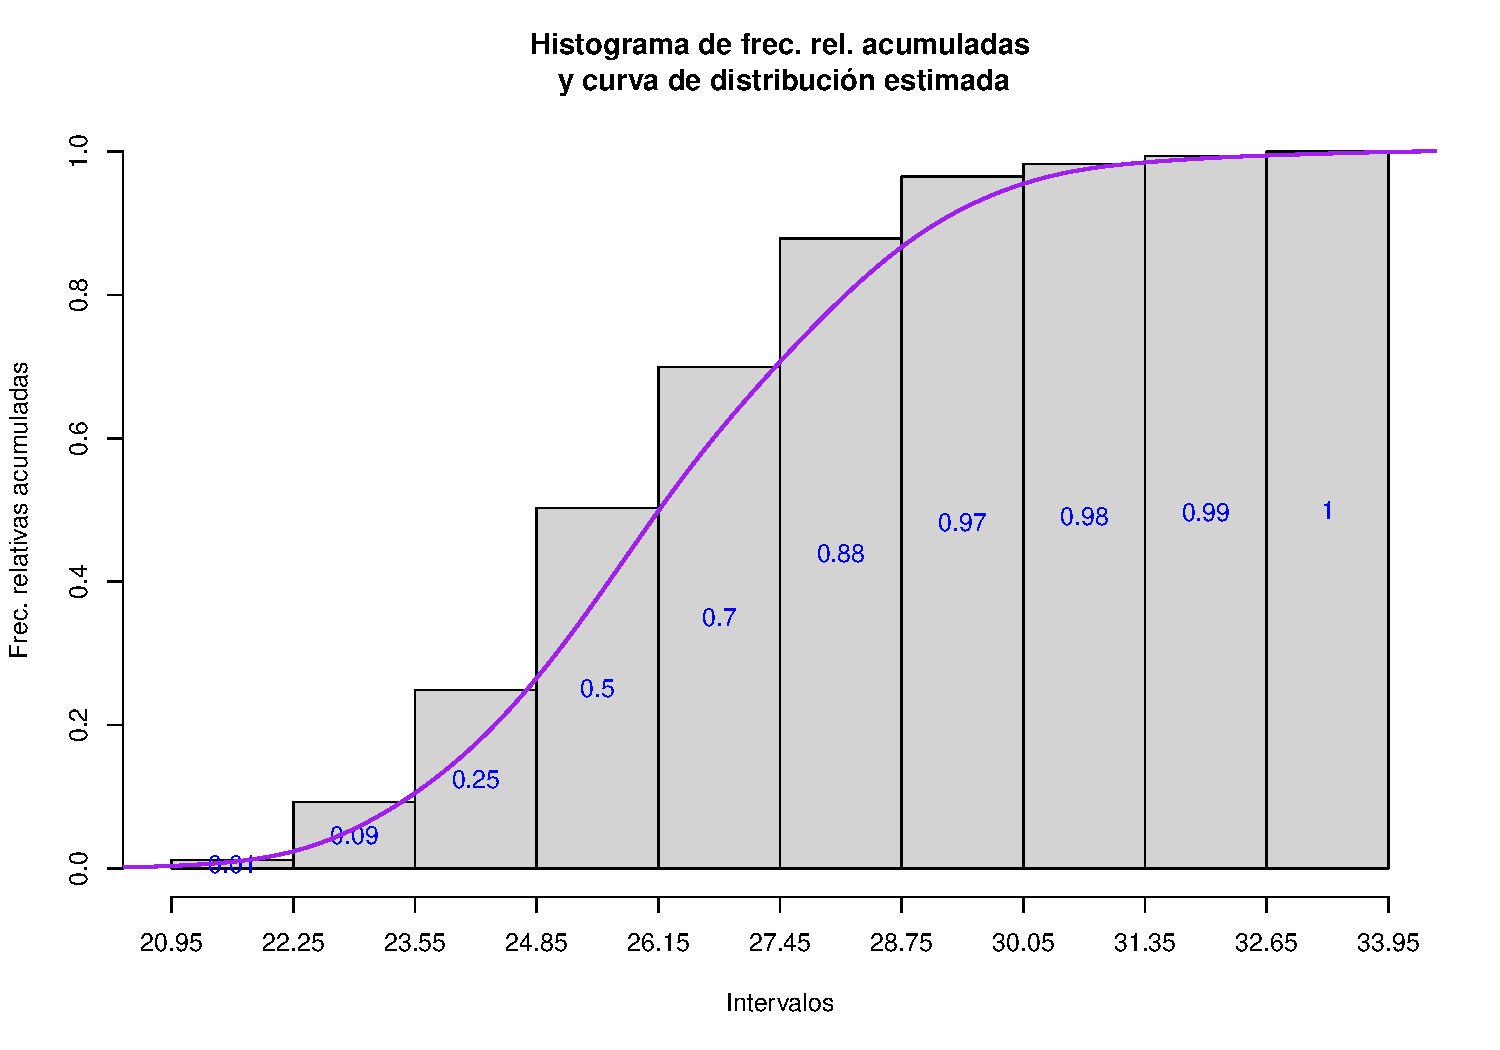
\includegraphics{Tema9.-Agrupacion_datos_cuantitativos_files/figure-beamer/unnamed-chunk-62-1.pdf}

\end{frame}

\end{document}
